\documentclass{report}

\usepackage{geometry}
\geometry{a4paper,total={170mm,257mm},left=20mm,top=20mm}
\usepackage[utf8]{inputenc}
\usepackage{amsmath}
\usepackage{amsfonts}
\usepackage{amsthm}
\usepackage{amssymb}
\usepackage{bm}
\usepackage{graphicx}
\usepackage{paralist}
\usepackage[dvipsnames]{xcolor}
\usepackage{caption}
\usepackage{subcaption}
\usepackage{hyperref}
\hypersetup{urlbordercolor=ForestGreen,linkbordercolor=RoyalPurple}
\usepackage{tikz}
\usetikzlibrary{positioning}
\usetikzlibrary{intersections}
\usepackage{algpseudocode}
\usepackage{algorithm}
\usepackage{titling}
\usepackage{pgfplots}
\usepackage{fontawesome5}

%%% Tento soubor obsahuje definice různých užitečných maker a prostředí %%%
%%% Další makra připisujte sem, ať nepřekáží v ostatních souborech.     %%%

%%% Drobné úpravy stylu

% Tato makra přesvědčují mírně ošklivým trikem LaTeX, aby hlavičky kapitol
% sázel příčetněji a nevynechával nad nimi spoustu místa. Směle ignorujte.
\makeatletter
\def\@makechapterhead#1{
  {\parindent \z@ \raggedright \normalfont
   \Huge\bfseries \thechapter. #1
   \par\nobreak
   \vskip 20\p@
}}
\def\@makeschapterhead#1{
  {\parindent \z@ \raggedright \normalfont
   \Huge\bfseries #1
   \par\nobreak
   \vskip 20\p@
}}
\makeatother

% Toto makro definuje kapitolu, která není očíslovaná, ale je uvedena v obsahu.
\def\chapwithtoc#1{
\chapter*{#1}
\addcontentsline{toc}{chapter}{#1}
}

% Trochu volnější nastavení dělení slov, než je default.
\lefthyphenmin=2
\righthyphenmin=2

% Zapne černé "slimáky" na koncích řádků, které přetekly, abychom si
% jich lépe všimli.
\overfullrule=1mm

%%% Makra pro definice, věty, tvrzení, příklady, ... (vyžaduje baliček amsthm)

\theoremstyle{plain}
\newtheorem{veta}{Věta}
\newtheorem{lemma}[veta]{Lemma}
\newtheorem{tvrz}[veta]{Tvrzení}

\theoremstyle{plain}
\newtheorem{definice}{Definice}
\newtheorem*{pozor}{Pozorování}
\newtheorem*{cvic}{Cvičení}
\newtheorem*{fakt}{Fakt}

\theoremstyle{remark}
\newtheorem*{dusl}{Důsledek}
\newtheorem*{pozn}{Poznámka}
\newtheorem*{prikl}{Příklad}

\theoremstyle{plain}
\newtheorem{thm}{Theorem}
%\newtheorem{lemma}[thm]{Lemma}
\newtheorem{claim}[thm]{Claim}

\theoremstyle{plain}
\newtheorem{defn}{Definition}
\newtheorem*{observ}{Observation}
\newtheorem*{exerc}{Exercise}
\newtheorem*{fact}{Fact}

\theoremstyle{remark}
\newtheorem*{cor}{Corollary}
\newtheorem*{rem}{Remark}
\newtheorem*{example}{Example}


%%% Prostředí pro důkazy

\newenvironment{dukaz}{
  \par\medskip\noindent
  \textit{Důkaz}.
}{
\newline
\rightline{$\qedsymbol$}
}

\newenvironment{myproof}{
	\par\medskip\noindent
	\textit{Proof}.
}{
	\newline
	\rightline{$\qedsymbol$}
}


%%% Prostředí pro sazbu kódu, případně vstupu/výstupu počítačových
%%% programů. (Vyžaduje balíček fancyvrb -- fancy verbatim.)

\DefineVerbatimEnvironment{code}{Verbatim}{fontsize=\small, frame=single}

%%% Prostor reálných, resp. přirozených čísel
\newcommand{\R}{\mathbb{R}}
\newcommand{\N}{\mathbb{N}}
\newcommand{\Z}{\mathbb{Z}}

%%% Užitečné operátory pro statistiku a pravděpodobnost
\DeclareMathOperator{\pr}{\textsf{P}}
\DeclareMathOperator{\E}{\textsf{E}\,}
\DeclareMathOperator{\var}{\textrm{var}}
\DeclareMathOperator{\sd}{\textrm{sd}}

%%% Příkaz pro transpozici vektoru/matice
\newcommand{\T}[1]{#1^\top}

%%% Vychytávky pro matematiku
\newcommand{\goto}{\rightarrow}
\newcommand{\gotop}{\stackrel{P}{\longrightarrow}}
\newcommand{\maon}[1]{o(n^{#1})}
\newcommand{\abs}[1]{\left|{#1}\right|}
\newcommand{\dint}{\int_0^\tau\!\!\int_0^\tau}
\newcommand{\isqr}[1]{\frac{1}{\sqrt{#1}}}

%%% Vychytávky pro tabulky
\newcommand{\pulrad}[1]{\raisebox{1.5ex}[0pt]{#1}}
\newcommand{\mc}[1]{\multicolumn{1}{c}{#1}}


% set up \maketitle to accept a new item
\predate{\begin{center}\placetitlepicture\large}
	\postdate{\par\end{center}}

% commands for including the picture
\newcommand{\titlepicture}[2][]{%
	\renewcommand\placetitlepicture{%
		\includegraphics[#1]{#2}\par\medskip
	}%
}
\newcommand{\placetitlepicture}{} % initialization


\usepackage{babel}

\title{Flows, paths and cuts}
\author{Tomáš Turek\thanks{Here are my notes from the course on Flows, paths and cuts. \INFO}}
\titlepicture[width=5in]{res/flow.pdf}
\date{\today}

\begin{document}
	\maketitle	
	\tableofcontents
	\chapter{Introducing}

Firstly we will start by the introduction to the main characters, which are firstly intersection defined graph classes and secondly characterization of chordal graphs.

\section{Intersection defined graph classes}

\begin{defn}
	The intersection graph of a set family $\mathcal{A}$ is the graph
	
	$$
	IG(\mathcal{A}) = (\mathcal{A}, \{ab : a \neq b, a \cap b \neq \emptyset, a, b \in \mathcal{A}\}).
	$$
\end{defn}

\begin{defn}
	Let $\mathcal{M}$ be a family of sets. We say that a graph $G$ is an intersection graph of (members of) $\mathcal{M}$ if $G$ is isomorphic to the graph $IG(\mathcal{A})$ for some family $\mathcal{A}$ whose all elements belong to $\mathcal{M}$. We write
	
	$$
	\mathcal{IG}(\mathcal{M}) = \{IG(\mathcal{A}) : \mathcal{A} \subseteq \mathcal{M}\}.
	$$
\end{defn}

\begin{observ}
	For every graph $G$ and every set family $\mathcal{M}, G \in \mathcal{IG}(\mathcal{M})$ if and only if there is a mapping $f : V (G) \to \mathcal{M}$ such that $uv \in E(G)$ iff $f(u) \cap f(v) \neq \emptyset$ holds true for all pairs of distinct vertices $u, v$ of $G$.
\end{observ}

\begin{observ}
	For every family $\mathcal{M}$ (containing at least one nonempty set), it holds that $\mathcal{IG}(\mathcal{M}$ contains all complete graphs and is hereditary (i.e., every induced subgraph of every graph from $\mathcal{IG}(\mathcal{M})$ also	belongs to $\mathcal{IG}(\mathcal{M})$).
\end{observ}

\subsection{Examples}

In many cases, the members of $\mathcal{M}$ are defined by their geometric shape. And in most of these cases, the members of $\mathcal{M}$ are arc-connected sets in the plane.

\begin{itemize}
	\item \textbf{Interval graphs} $\text{INT} = \mathcal{IG}(\{\text{intervals on a line}\})$
	\item \textbf{Circle graphs} $\text{CIR} = \mathcal{IG}(\{\text{chords of a circle}\})$
	\item \textbf{Circular arc graphs} $\text{CA} = \mathcal{IG}(\{\text{arcs on a circle}\})$
	\item \textbf{Permutation graphs} $\text{PER} = \mathcal{IG}(\{\text{segments connecting two parallel lines}\})$
	\item \textbf{Function graphs} $\text{FUN} = \mathcal{IG}(\{\text{curves connecting two parallel lines}\})$
	\item \textbf{Polygon circle graphs} $\text{PC} = \mathcal{IG}(\{\text{polygons inscribed in a circle}\})$
	\item \textbf{Segment graphs} $\text{SEG} = \mathcal{IG}(\{\text{straight-line segments in the plane}\})$
	\item \textbf{Convex graphs} $\text{CONV} = \mathcal{IG}(\{\text{convex sets in the plane}\})$
	\item \textbf{String graphs} $\text{STRING} = \mathcal{IG}(\{\text{curves in the plane}\})$
\end{itemize}

\begin{figure}[!ht]\centering
	\begin{subfigure}{0.45\textwidth}\centering
		
\begin{tikzpicture}
			\draw[line width = 3] (0,0) -- (6,0);
			\draw[line width = 4, color = cyan] (1, .12) -- (3, .12);
			\draw[line width = 4, color = violet] (4, .12) -- (5, .12);
			\draw[line width = 4, color = orange] (2, .25) -- (5.5, .25);
		\end{tikzpicture}
		\caption{Drawn intervals.}
	\end{subfigure}
	\begin{subfigure}{0.45\textwidth}\centering
		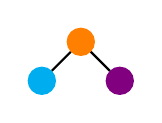
\begin{tikzpicture}[node distance={7mm}, thick, main/.style = {draw, circle, fill}]
			\node[main, color=cyan] (C) {};
			\node[main, color=orange] (O) [above right of=C] {};
			\node[main, color=violet] (V) [below right of=O] {};
			\draw (O) edge (V);
			\draw (C) edge (O);
		\end{tikzpicture}
		\caption{Corresponding graph.}
	\end{subfigure}
	\caption{Example of a graph from INT class.}
\end{figure}

\begin{figure}[!ht]\centering
	\begin{subfigure}{0.45\textwidth}\centering
		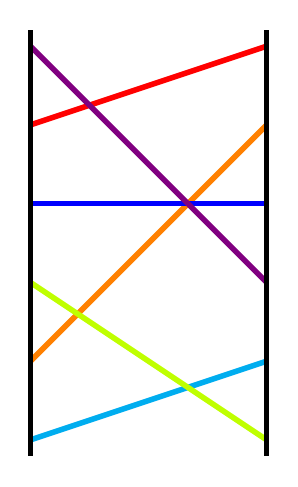
\begin{tikzpicture}[node distance={9mm}, thick, main/.style = {draw, circle}]
			\draw[line width = 2, color = cyan] (0,1) -- (3,2);
			\draw[line width = 2, color = orange] (0,2) -- (3,5);
			\draw[line width = 2, color = lime] (0,3) -- (3,1);
			\draw[line width = 2, color = blue] (0,4) -- (3,4);
			\draw[line width = 2, color = red] (0,5) -- (3,6);
			\draw[line width = 2, color = violet] (0,6) -- (3,3);
			\draw[line width = 2] (0,.8) -- (0,6.2);
			\draw[line width = 2] (3,.8) -- (3,6.2);
		\end{tikzpicture}
		\caption{Drawn permutations.}
	\end{subfigure}
	\begin{subfigure}{0.45\textwidth}\centering
		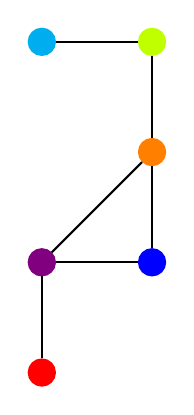
\begin{tikzpicture}[node distance={14mm}, thick, main/.style = {draw, circle, fill}]
			\node[main, color=cyan] (1) {};
			\node[main, color=lime] (2) [right of=1] {};
			\node[main, color=orange] (3) [below of=2] {};
			\node[main, color=blue] (4) [below of=3] {};
			\node[main, color=violet] (5) [left of=4] {};
			\node[main, color=red] (6) [below of=5] {};

			\draw (1) edge (2);
			\draw (2) edge (3);
			\draw (3) edge (4);
			\draw (3) edge (5);
			\draw (4) edge (5);
			\draw (5) edge (6);
		\end{tikzpicture}
		\caption{Corresponding graph.}
	\end{subfigure}
	\caption{Example of a graph from PER class.}
\end{figure}

\section{Chordal graphs}

\begin{defn}
	A graph is \textbf{chordal} if it does not contain any cycle of length greater than three as an induced subgraph.
\end{defn}

\begin{defn}
	A vertex $u$ of a graph $G$ is \textbf{simplicial} if $G[N_G(u)]$ is a clique.
\end{defn}

\begin{defn}[PES \PES]
	A \textbf{perfect elimination scheme} for a graph $G$ is a linear ordering $u_1, u_2, \dots, u_n$ of its vertices such that for every $i, u_i$ is simplicial in the induced subgraph $G[\{u_1, u_2, \dots, u_i\}]$.
\end{defn}

\begin{lemma}
	Every minimal vertex cut in a chordal graph induces a clique.
\end{lemma}

\begin{proof}
	Let $A \subset V(G)$ be a minimal vertex cut, and suppose $u, v$ be two vertices of $A$. These vertices	are connected by a path in each component of $G \setminus A$. If $u$ and $v$ were not adjacent, a pair of shortest such paths would give rise to an induced cycle of length greater than 3 in $G$.
\end{proof}

\begin{lemma}
	Every chordal graph, which is not a complete graph, contains two nonadjacent simplicial vertices.
	\label{lemma-r2}
\end{lemma}

\begin{proof}
	By induction. If $G$ is a complete graph, the claim of the lemma is fulfilled. If $G$ is not complete, it has a vertex cut, say $A$. Let $B$ be a connected component of $G \setminus A$, and set $G_1 = G[B \cup A]$ and $G_2 = G \setminus B$. By induction hypothesis, each of $G_1, G_2$ is either complete or has two nonadjacent simplicial vertices. Thus each of them has a simplicial vertex which does not belong to $A$. Each of	these is then also simplicial in entire $G$, and they are clearly nonadjacent.
\end{proof}

\begin{cor}
	Every nonempty chordal graph contains a simplicial vertex.
\end{cor}

\begin{defn}[Clique-tree decomposition]
	A \textbf{clique-tree decomposition} of a graph $G$ is a tree $T = (\mathcal{Q}, F)$, with $\mathcal{Q}$ being the set of all maximal cliques of $G$, such that for every vertex $u \in V(G)$, the subgraph $T[\{Q : u \in Q \in \mathcal{Q}\}]$ is connected.
\end{defn}

\textbf{Warning!! The vertex set of a clique-tree decomposition of a graph G is uniquely defined, but not necessarily the edge set!!}

\begin{thm}
	For any graph $G$, the following statements are equivalent:
	
	\begin{enumerate}
		\item $G$ is chordal,
		\item $G$ allows a PES.
		\item $G$ has a clique-tree decomposition, and
		\item $G$ is an intersection graph of subtrees of a tree.
	\end{enumerate}
\end{thm}

\begin{proof}
	"$1. \Rightarrow 2.$" By induction on the number of vertices, using Lemma \ref{lemma-r2}.
	
	"$2. \Rightarrow 3.$" By induction on the number of vertices again. Suppose $G' = G \setminus v_n$ has a clique-tree	$T = (\mathcal{Q}' , F')$. If $Q' = N_G (v_n) \in \mathcal{Q}'$ , then $Q = N_G [v_n]$ is a maximal clique in $G, \mathcal{Q} = (\mathcal{Q}' \setminus \{Q'\}) \cup \{Q\}$ and $T = (\mathcal{Q}, F)$ is a clique-tree for $G$, where $F = (F' \setminus \{Q' P : P \in \mathcal{Q}'\}) \cup \{QP : Q'P \in F'\}$. If, on the other hand, $Q' = N_G(v_n) \notin \mathcal{Q}'$ , then $\mathcal{Q} = \mathcal{Q}' \cup N_G [v_n]$ and $(\mathcal{Q}, F' \cup N_G [v_n]P)$ is a clique-tree for $G$ for any $P \in \mathcal{Q}'$ such that $N_G (v_n) \subset P$.
	
	"$3. \Rightarrow 4.$" Given a clique-tree decomposition $T = (\mathcal{Q}, F)$, define $T_u = T [\{Q : u \in Q \in \mathcal{Q}\}]$ for $u \in V(G)$. Clearly $V(T_u) \cap V(T_v) \neq \emptyset$ iff $u$ and $v$ belong to the same maximal clique of $G$, which happens if and only if $u$ and $v$ are adjacent in $G$.
	
	"$4. \Rightarrow 1.$" Let $G$ be the intersection graph of a collection $\{T_u\}_{u \in V(G)}$ of subtrees of a tree $T$. Suppose $v_1, v_2, \dots, v_k$ be an induced cycle in $G$, with $k > 3$. Then the subtrees $T_{v_1}$ and $T_{v_3}$ are vertex disjoint, and hence there is an edge $e \in E(T)$ which lies on every path connecting $T_{v_1}$ and $T_{v_3}$ in $T$ . This edge separates $T$ into $T_1$ and $T_2$ such that $T_{v_1}$ and $T_{v_3}$ belong to different components of $T \setminus e$, say, $T_{v_1} \subseteq T_1$ and $T_{v_3} \subseteq T_2$. One can show by induction on $i$ that for every $i \geq 3$, $T_{v_i} \subseteq T_2$. But then $T_{v_k}$ and $T_{v_1}$ must be disjoint, contradicting the assumption that $v_1 v_k \in E(G)$.
\end{proof}

\begin{cor}
	Chordal graphs are perfect (i.e., $\chi(H) = \omega(H)$ for every induced subgraph $H$ of $G$).
\end{cor}

\begin{proof}
	Consider a PES $u_1, u_2, \dots, u_n$ for $G$ and color the vertices from $u_1$ to $u_n$ by the First Fit Method (we try to use minimal color if we cannot use any of them, create a new color).
\end{proof}
	\chapter{Multi-commodity problem}

On a graph $G = (V,E)$ and $k$ tuples $(s_{1}, t_{1}), (s_{2}, t_{2}), \dots, (s_{k}, t_{k}) \in V^{2}$ known as \textbf{commodities} we can also define a network and a flow. Same as before we have a capacity $c: E \to \R_{0}^{+}$. These commodities are shared on the same resources.

We may define $\mathcal{P}_{i}$ as all paths between $s_{i}$ and $t_{i}$. And also $\mathcal{P} := \bigcup_{i = 1}^{k} \mathcal{P}_{i}$.

For a single commodity flow problem we could define a \textit{linear program} (LP):

$$
\begin{aligned}
	\max \sum_{p \in \mathcal{P}_{st}} f_{p} \\
	\sum_{p: e \in p \in \mathcal{P}_{st}} f_{p} \leq c(e) &\quad \forall e \in E\\
	f_p \geq 0 &\quad \forall p \in \mathcal{P}_{st}
\end{aligned}
$$

From this we may define a linear program denoted as \textbf{LP1} for multi commodity problem.

$$
\begin{aligned}
	\max \sum_{p \in \mathcal{P}} f_{p} = \sum_{i = 1}^{k} \sum_{p \in \mathcal{P}_{i}} f_{p} \\
	\sum_{j = 1}^{k} \sum_{p: e \in p \in \mathcal{P}_{j}} f_{p} \leq c(e) & \quad \forall e \in E\\
	f_p \geq 0 & \quad \forall p \in \mathcal{P}
\end{aligned}
$$

Alternatively we could define it by a single variables for flows on each edge. For multi commodity problem we would have $k$ flows which adds up to one single flow. Thus we can see that the problem is in $P$ (polynomial).

\section{Multi cut problem}

As cuts for single flow we may define somewhat similiar definition. Such that for every $i$ the pair $s_{i}$ and $t_{i}$ are not connected by any path. We will also look at a linear program which will be denoted as \textbf{LP2}.

$$
\forall e : x_{e} =
\left\{
\begin{array}{rl}
	1 & e \text{ in cut} \\
	0 & \text{otherwise}	
\end{array}
\right.
$$

$$
\begin{aligned}
	\min \sum_{e \in E} x(e) c(e) & \quad =: \Phi \quad \text{(notation for further use)}\\
	\sum_{e \in p} x(e) \geq 1 &\quad \forall i \in [k] \ \forall p \in \mathcal{P}_{i}\\
	x(e) \in \{0, 1\} &\quad \forall e \in E(G)  \quad \text{(ILP)}\\
	x(e) \geq 0 &\quad \forall e \in E(G) \quad \text{(LP)} 
\end{aligned}
$$

First ILP is integer linear program which is generally NP hard. Thus we will look on the relaxation of LP program. We may observe that we don't need to specify that $x(e) \leq 1$ due to the minimality.

Now we may see that indeed \textbf{LP1} and \textbf{LP2} are dual programs. Thus resulting in knowing that the maximum flow is the same as minimum fractional cut.

\section{Example}

Before we continue we will take a look at a simple example (\ref{example}). The graph is as follows. All capacities are equal to $1$.

\begin{figure}[!h]\centering
	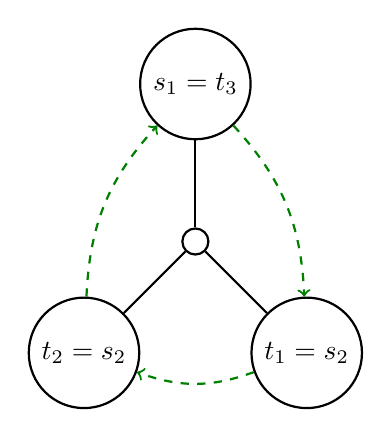
\begin{tikzpicture}[node distance={20mm}, thick, main/.style = {draw, circle}]
		\node[main] (1) {$s_{1} = t_{3}$};
		\node[main] (4) [below of=1] {};
		\node[main] (2) [below right of=4] {$t_{1} = s_{2}$};
		\node[main] (3) [below left of=4] {$t_{2} = s_{2}$};
		\draw (1) -- (4);
		\draw (4) -- (2);
		\draw (4) -- (3);
		\draw[dashed, bend left = 20, color = Green, ->] (1) edge (2);
		\draw[dashed, bend left = 20, color = Green, ->] (2) edge (3);
		\draw[dashed, bend left = 20, color = Green, ->] (3) edge (1);
	\end{tikzpicture}
	\caption{Example graph. With \textcolor{Green}{visualized commodities}.}
	\label{example}
\end{figure}

We may observe that the max flow is $|f| = \frac{3}{2}$ because we can put $\frac{1}{2}$ on every edge. Then multi-cut is $2$ since we need to remove always at least two edges. But minimum fractional multi-cut is only $\frac{3}{2}$ because we only have to "cut" half of each edge. Thus it is the exact same result as max flow.

\section{Preparation for algorithm}

We will show an algorithm which will give an approximate result of a multi-cut problem. We may look at it like we would cut off some parts of the graph which are close to the sources and continue.

Given $\bar{G} = \left(\bar{V}, \bar{E}\right), (s_{i}, t_{i}), k, c: E \to \R_{0}^{+}$ and solution $x$ of \textbf{LP2}. We define:

$$
B_{x}(s_{i}, r) := \left\{u \in \bar{V} | d_{x} (s_{i}, u) \leq r\right\}
$$

As a ball around $s_{i}$ with diameter w.r.t $x$. $d_{x} (s_{i}, u) :=$ the length of the shortest $s_{i}u$ path in $\bar{G}$ w.r.t. the edge length $x(e)$.

$$
\delta (B_{x}(s_{i}, r)) = \left\{\{u,v\} \in \bar{E} : |\{u,v\} \cap B_{x}(s_{i}, r)| = 1\right\}
$$

$$
V_{x}(s_{i}, r) = \frac{\Phi}{k} + \sum_{\{u,v\} \in \bar{E}, u,v \in B_{x}(s_{i},r)} c(e)x(e) + \sum_{\{u,v\} \in \delta(B_{x}(s_{i},r)): u \in B_{x}(s_{i},r)} c(e) (r - d_{x}(s_{i}, u))
$$

This we call a volume of a ball. We will denoted as a function $f(r)$ for $r$. The last sum is of all edges which are only partly inside the ball. Next we also define the following.

$$
C_{x}(s_{i}, r) = \sum_{\{u,v\} \in \delta(B_{x}(s_{i},r))} c(u,v)
$$

This will be denoted as a function $g(r)$. We may see some really nice properties these functions have. For instance $f(r)$ is a growing function which is increasing linearly and then it jumps to another point. On the other hand $g(r)$ is constant on some parts and then it jumps to a certain point, these jumps are for both function in the exact same spots. Next we can see that for some nice points it holds that $f'(r) = g(r)$. These nice points are all but the jumps.

\begin{lemma}
	For each $i \in [n]$ s.t. $s_{i}, t_{i} \in \bar{V}$ there exist $r \in (0, 1/2)$ s.t.
	
	$$
	\frac{C_{x}(s_{i}, r)}{V_{x}(s_{i},r)} \leq 2 \ln 2k.
	$$
	\label{multi cut lemma}
\end{lemma}

\begin{proof}
	By contradiction. For fixed $i$ $\forall r \in (0, 1/2)$, $\frac{f'(r)}{f(r)} > 2 \ln 2k$. We will have $r_{0} = 0 < r_{1} < r_{2} < \dots < r_{l-1} < 1/2 = r_{l}$ which are the values where $f(r)$ is not continuous (there are these "jumps"). First we consider $r \in (r_{j}, r_{j+1})$ for some $j$.
	
	$$
	\frac{f'(r)}{f(r)} = \left( \ln f(r)\right)'
	$$
	
	So for the contradiction $\forall r \in (r_{j}, r_{j+1})$, $\left( \ln f(r)\right)' > 2 \ln 2k$. We will compute the integral over all of these values. We may see that the right side is just a constant so we get
	
	$$
	\int_{r_{j}}^{r_{j+1}} \left( \ln f(r)\right)' > (r_{j+1} - r_{j}) 2 \ln 2k.
	$$
	
	In $r_{j+1}$ there may be jump so we instead take the $\lim_{r \to r_{j+1}^{-}} f(r) = f^{-}(r_{j+1})$. Note that $f^{-}(r_{j+1}) \leq f(r_{j+1})$.
	
	$$
	\ln f(r_{j+1}) - \ln f(r_{j}) \geq \ln f^{-}(r_{j+1}) - \ln f(r_{j}) = \int_{r_{j}}^{r_{j+1}} \left( \ln f(r)\right)' > (r_{j+1} - r_{j}) 2 \ln 2k.
	$$
	
	Now we sum our inequality over all intervals $(r_{j}, r_{j+1}), j = 0, \dots, l$. We will only have the very ends because the rest will be once added and once removed.
	
	$$
	\begin{aligned}
		\sum_{j = 0}^{l-1} \left( \ln f(r_{j+1}) - \ln f(r_{j}) \right) &> \sum_{j = 0}^{l-1} (r_{j+1} - r_{j}) 2 \ln 2k\\
		\ln f(r_{l}) - \ln f(r_{0}) &> (r_{l} - r_{0}) 2 \ln 2k\\
		\ln f(1/2) - \ln f(0) &> \ln 2k\\
		\ln \frac{f(1/2)}{\frac{\Phi}{k}} &> \ln 2k\\
		\frac{f(1/2)}{\frac{\Phi}{k}} &> 2k\\
		f(1/2) &> 2 \Phi
	\end{aligned}
	$$
	
	As the volume of the entire pipe system is at most $2 \Phi$ it means that we have a contradiction.
\end{proof}

Note that choosing $1/2$ is not necessary for the proof, but for the algorithm to work. Because if we choose $1/2$ it means that no $s_{j}, t_{j}$ will both be in a ball for the index $i$. That is because the length w.r.t $x$ of paths from $s_{j}$ to $t_{j}$ need to be at least $1$.

\section{Pipe cut algorithm}

\begin{algorithm}[!h]
	\caption{Pipe cut algorithm}
	\begin{algorithmic}[1]
		\Require $\bar{G} = (\bar{V}, \bar{E})$.
		\Ensure $F$ multi cut.
		\State $F \gets \emptyset$
		\For{$i = 1 \dots k$}
			\If{$s_{i}-t_{i}$ are still connected in $\left(\bar{V}, \bar{E} \setminus F\right)$}
				\State Choose $r \in (0, 1/2)$ by Lemma \ref{multi cut lemma}.
				\State $F \gets F \cup \delta(B_{x}(s_{i}, r))$
				\State Remove edges inside $B_{x}(s_{i}, r)$ and $\delta(B_{x}(s_{i}, r))$.
			\EndIf
		\EndFor \\
		\Return $F$
	\end{algorithmic}
\end{algorithm}



There are few things to talk about. To get $r$ we will check all "almost ends" of all intervals. The time complexity is polynomial since everything that is inside the code is polynomial. Correctness of the algorithm is easily observable since no pair $s_{i},t_{i}$ is inside some other ball and all balls will separate pairs $s_{j}, t_{j}$. Other thing to consider is what is the approximation ratio?

\begin{thm}
	Approximation ratio of the Pipe cut algorithm is $O(\log k)$.
\end{thm}

\begin{proof}
	Lets define $C_{i}$ as the cost of the cut of the ball from iteration $i$ and $V_{i}$ as the volume of it. We know that $C_{i} \leq 2 \ln 2k \cdot V_{i}$.
	
	$$
	\sum_{i} C_{i} \leq 2 \ln 2k \sum_{i}V_{i} \leq 2 \ln 2k \cdot 2 \Phi = 4 \ln 2k \cdot \Phi = O (\log k) \Phi
	$$
\end{proof}

For a single commodity we know that max flow $=$ min cut. Where $\leq$ is trivial and $\geq$ is a little harder. This is a case of \textbf{exact duality}. On the other hand we already shown that this doesn't hold for multi-commodity, but what if we can define \textbf{approximate duality}.

\begin{cor}
	Max flow $\leq$ min cut $\leq O(\log k)$ max flow. For multi-commodity case.
\end{cor}

\begin{proof}
	Because of the duality of LP1 and LP2 we know that max flow is the same as min fractional multi-cut. And because of the algorithm we know that the fractional multi-cut is in $O(\log k)$.
\end{proof}

\section{How to solve LP}

There is still a problem with our LP which can have up to exponential many of constraints. But this can be solved fast by using \textbf{Ellipsoid algorithm} on $A x \leq b$. Only thing it needs is an \textbf{ORACLE} which is that for given $\bar{x}$, check whether $A\bar{x} \leq b$ and if not return a particular violated constraint.

In our case \textbf{ORACLE} is for each $i$ find the shortest $s_{i}-t_{i}$ path w.r.t $\bar{x}$. This can be either $\geq 1$ and we are happy or $< 1$ then this constraint is violated.

\section{Is there any better approximation?}

We will show that indeed this approximation is the best we can get. Firstly we will define a new property of graphs.

\begin{defn}
	A graph $G = (V,E)$ is an \textbf{$\alpha$-expander} if $\forall S \subseteq V, |S| \leq \frac{n}{2}, \delta(S) \leq \alpha |S|$.
\end{defn}

We take as granted that it holds: $3$-regular $\alpha$-expanders exist for $\alpha > 0$. Now lets observe an example on the picture \ref{3-regular} that at most $1 + 3 \cdot 2^{l-1}$ vertices are reachable by a path of length $\leq l$.

\begin{figure}[!h] \centering
	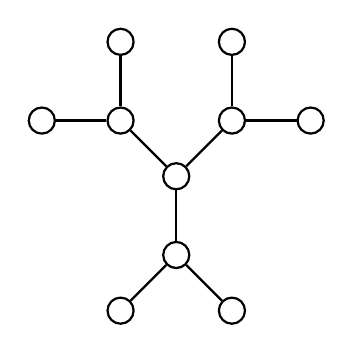
\begin{tikzpicture}[node distance={10mm}, thick, main/.style = {draw, circle}]
		\node[main] (1) {};
		\node[main] (2) [below of=1] {};
		\node[main] (3) [above right of=1] {};
		\node[main] (4) [above left of=1] {};
		\node[main] (5) [below left of=2] {};
		\node[main] (6) [below right of=2] {};
		\node[main] (7) [above of=3] {};
		\node[main] (8) [right of=3] {};
		\node[main] (9) [above of=4] {};
		\node[main] (10) [left of=4] {};
		\draw (1) -- (4);
		\draw (1) -- (2);
		\draw (1) -- (3);
		\draw (2) -- (5);
		\draw (2) -- (6);
		\draw (3) -- (7);
		\draw (3) -- (8);
		\draw (4) -- (9);
		\draw (4) -- (10);
	\end{tikzpicture}
	\caption{How to get the upper bound. The graph continue and it is 3-regular.}
	\label{3-regular}
\end{figure}

If we take $l = \log_{2} \frac{n-2}{6} + 1$ so with the upper bound we get $1 + 3 \cdot \frac{n-2}{6} = 1 + \frac{n-2}{2} = \frac{n}{2}$. And also we define an instance of multi-commodity problem: $T = \left\{\{u,v\} | d(u,v) > l\right\}$. A unit of flow consumes $\geq l$ units of volume of the entire system. Thus $|E| = O(n)$. Therefore max flow $\leq O(\frac{n}{l}) = O(\frac{n}{\log n})$. But for min cut we take the optimum $F \subseteq E$. Every path in $G = (V, E \setminus F)$ is $\leq \frac{n}{2}$ so min cut is $\Theta(n)$. Thus it is indeed tight.
	\chapter{The Sparsest cut problem}

Same as before we have an undirected graph $G = (V,E)$ and $k$-pairs of sources and targets $(s_{1},t_{1}), (s_{2}, t_{2}), \dots,\\ (s_{k}, t_{k}) \in V^{2}$. But we will introduce a new parameters $d_{1}, d_{2}, \dots, d_{k} \in \R^{+}$ called \textbf{demands}.

Firstly we will take a look at linear program for solving this problem for $k = 1$.

$$
\begin{aligned}
	\max f \\
	\sum_{p \in \mathcal{P}_{st}} x_{p} \geq f \cdot d_{1} \\
	\sum_{p : e \in p \in \mathcal{P}_{st}} x_{p} \leq c(e) & \quad \forall e \in E\\
	x \geq 0
\end{aligned}
$$

Where $\mathcal{P}_{st}$ are all paths between $s$ and $t$. We may see that the optimum of the max flow is the same as this optimum just divided by $d_{1}$. We will denote $\mathcal{P}_{i} = \mathcal{P}_{s_{i}, t_{i}}$.

\section{Concurrent multicommodity flow}

Thus we are getting this LP for all $k$ commodities and $k$ demands.

$$
\begin{aligned}
	\max f \\
	\sum_{p \in \mathcal{P}_{i}} x_{p} \geq f \cdot d_{i} & \quad \forall i \in [k]\\
	\sum_{i = 0}^{k} \sum_{p: e \in p \in \mathcal{P}_{i}} x_{p} \leq c(e) & \quad \forall e \in E\\
	x \geq 0
\end{aligned}
$$

We will take a look at the matrix of this LP and after that find a dual program. But firstly we modify $\sum_{p \in \mathcal{P}_{i}} x_{p} \geq f \cdot d_{i}$ to $f \cdot d_{i} - \sum_{p \in \mathcal{P}_{i}} x_{p} \leq 0$. Then the matrix is as follows:

$$
\begin{matrix}
	  & f     &    & \mathcal{P}_{1} &       &    & \mathcal{P}_{2} &       & \dots \\
	1 & d_{1} & -1 & -1              & \dots &  0 & \dots           & 0     & \dots \\
	2 & d_{2} & 0  &  0              & \dots & -1 & -1              & \dots & 0     \\
	\vdots  \\
	k & d_{k} & 0  &  0              & \dots & 0 & 0               &  0    & \dots \\
	e_{1} & 0     & 1  &  0              &       & 1 & 0               &  0    & \dots \\
	\vdots \\
	e_{|E|} & 0     & 0  &  1              &       & 1 & 0               &  1    & \dots \\
\end{matrix}
$$

Where for the first $k$ lines are $\leq 0$ and for edges it is $\leq c(e)$. We visualized the matrix and thus we can make the dual. We will have variables $x_{e}$ for edges and $y_{i}$ for $i \in [k]$. Thus the dual is:

$$
\begin{aligned}
	\min \sum_{e \in E} x_{e}c(e) \\
	\sum_{i = 0}^{k} y_{i}d_{i} \geq 1 \\
	\sum_{e \in p} x_{e} -y_{i} \geq 0 & \quad \forall i \in [k] \forall p \in \mathcal{P}_{i}\\
	x,y \geq 0
\end{aligned}
$$

\begin{defn}
	For $S \subseteq V$ we define $\delta(S) = \{\{u,v\} \in E : |\{u,v\} \cap S| = 1\}$ and then $I(S) = \{i \in [k] : |\{s_{i}, t_{i}\} \cap S| = 1\}$. Then the \textbf{sparsity} of $S$ is
	
	$$
	\rho(S) = \frac{\sum_{e \in \delta(S)}c(e)}{\sum_{i \in I(S)} d_{i}}
	$$
\end{defn}

\begin{example}
	We will have a simple example where all capacities are 1 and all demands are 1. So we have the graph \ref{example-sparse}. Note that there are 4 pairs of $s_i, t_i$ which can be seen by their demands.
	
	\begin{figure}[!h]\centering
		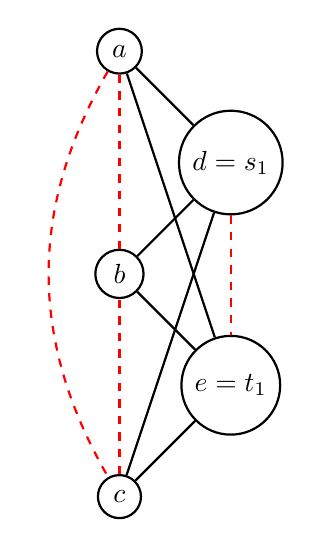
\begin{tikzpicture}[node distance={20mm}, thick, main/.style = {draw, circle}]
			\node[main] (1) {$a$};
			\node[main] (2) [below right of=1] {$d = s_{1}$};
			\node[main] (3) [below left of=2] {$b$};
			\node[main] (4) [below right of=3] {$e = t_{1}$};
			\node[main] (5) [below left of=4] {$c$};
			\draw (1) -- (2);
			\draw (1) -- (4);
			\draw (3) -- (2);
			\draw (3) -- (4);
			\draw (5) -- (2);
			\draw (5) -- (4);
			\draw [red, dashed] (1) -- (3);
			\draw [red, dashed] (5) -- (3);
			\draw [red, dashed] (2) -- (4);
			\path (1) edge [bend right, red, dashed] (5);
		\end{tikzpicture}
		\caption{Sparse cut example.}
		\label{example-sparse}
	\end{figure}
	
	The demands are the red edges. We may see that if we choose $S = \{c, e\}$ then $\sum_{e \in \delta(S)} c(e) = 3$ and $\sum_{i \in I(S)} d_{i} = 3$ therefore $\rho(S) = 1$.
	
	We may see that each pair $s_{i}$ $t_{i}$ consumes at least 2 units of a flow of the network for a single unit of the flow. Then we set $f$ as a max flow and see what we get. For example for paths $\mathcal{P}_{1} = \{(d,a,e) = p_{1}, (d,b,e) = p_{2}, (d,c,e) = p_{3}\}$. $x_{p_{1}} + x_{p_{2}} + x_{p_{3}} \geq f \cdot d_{1} = f$. Thus the total volume consumed by a flow with objective value $f$ is $\geq k 2 f = 8f$. Total volume of $G$ is 6. Therefore $f \leq \frac{6}{8} = \frac{3}{4}$.
	
	Maybe we can ask if there exist such a flow with this volume. We can obtain it by pushing $\frac{1}{4}$ from $d$ to $e$ on each path. And $\frac{3}{8}$ between all other pairs on all paths. All edges are not over their capacities and we get $\frac{3}{4}$ for all demands. Therefore we obtain following graph on picture \ref{max sparsest cut}. Hence there are 3 paths from $d$ to $e$ so in total it is $3/4$ and there two paths from $a$ to $b$ (and other pairs are same) therefore in total $6/8 = 3/4$.
	
	\begin{figure}[!h]\centering
		\begin{subfigure}{0.45\textwidth}\centering
			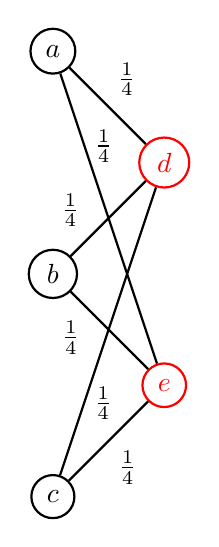
\begin{tikzpicture}[node distance={20mm}, thick, main/.style = {draw, circle}]
				\node[main] (1) {$a$};
				\node[main, color = red] (2) [below right of=1] {$d$};
				\node[main] (3) [below left of=2] {$b$};
				\node[main, color = red] (4) [below right of=3] {$e$};
				\node[main] (5) [below left of=4] {$c$};
				\draw (1) -- (2) node[midway, above right] {$\frac{1}{4}$};
				\draw (1) -- (4) node[near start, right] {$\frac{1}{4}$};
				\draw (3) -- (2) node[near start, above left] {$\frac{1}{4}$};
				\draw (3) -- (4) node[near start, below left] {$\frac{1}{4}$};
				\draw (5) -- (2) node[near start, right] {$\frac{1}{4}$};
				\draw (5) -- (4) node[midway, below right] {$\frac{1}{4}$};
			\end{tikzpicture}
			\caption{Paths from $d$ to $e$.}
		\end{subfigure}
		\begin{subfigure}{0.45\textwidth}\centering
			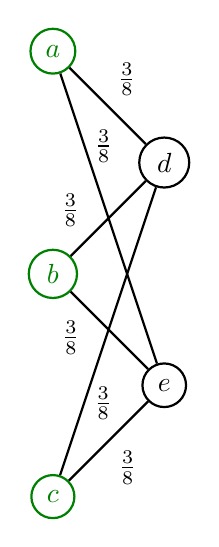
\begin{tikzpicture}[node distance={20mm}, thick, main/.style = {draw, circle}]
				\node[main, color = Green] (1) {$a$};
				\node[main] (2) [below right of=1] {$d$};
				\node[main, color = Green] (3) [below left of=2] {$b$};
				\node[main] (4) [below right of=3] {$e$};
				\node[main, color = Green] (5) [below left of=4] {$c$};
				\draw (1) -- (2) node[midway, above right] {$\frac{3}{8}$};
				\draw (1) -- (4) node[near start, right] {$\frac{3}{8}$};
				\draw (3) -- (2) node[near start, above left] {$\frac{3}{8}$};
				\draw (3) -- (4) node[near start, below left] {$\frac{3}{8}$};
				\draw (5) -- (2) node[near start, right] {$\frac{3}{8}$};
				\draw (5) -- (4) node[midway, below right] {$\frac{3}{8}$};
			\end{tikzpicture}
			\caption{Flows between the rest of the pairs.}
		\end{subfigure}
		\caption{Maximal sparsest flow $f$ in $G$.}
		\label{max sparsest cut}
	\end{figure}
\end{example}

\begin{defn}
	Now $F \subseteq E : I(F) = \{i \in [k] : s_{i}, t_{i} \text{ are in different components in } (V, E \setminus F)\}$. And \textbf{sparsity} of $F$ is defined as
	
	$$
	\rho(F) = \frac{\sum_{e \in F}c(e)}{\sum_{i \in I(F)} d_{i}}
	$$
\end{defn}

\begin{lemma}
	$\min_{S \subseteq V} \rho(S) = \min_{F \subseteq E} \rho(E)$.
\end{lemma}

\begin{proof}
	The $\geq$ inequality can be easily seen if we set $F$ to be $\delta(S)$. Now we need to show the other inequality. For given $F \subseteq E$, let $S_{1}, \dots S_{l}$ be the components of connectivity of $(V, E \setminus F)$. For that we will proof that $\min_{i \in [l]} \rho(S_{i}) \leq \rho(F)$. This will be shown by a contradiction. Assume $\forall i$:
	
	$$
	\begin{aligned}
		\frac{\sum_{e \in \delta(S_{i})}c(e)}{\sum_{j \in I(S_{i})} d_{j}} &> \frac{\sum_{e \in F}c(e)}{\sum_{j \in I(F)} d_{j}}\\
		\sum_{e \in \delta(S_{i})}c(e) &> \rho(F) \cdot \sum_{j \in I(S_{i})} d_{j}
	\end{aligned}
	$$
	
	Now we sum all $i$ inequalities.
	
	$$
	\sum_{i = 1}^{l} \sum_{e \in \delta(S_{i})}c(e) > \rho(F) \cdot \sum_{i = 1}^{l} \sum_{j \in I(S_{i})} d_{j}
	$$

	We can see that $\sum_{i = 1}^{l} \sum_{e \in \delta(S_{i})}c(e) = 2 \sum_{e \in F} c(e)$ because all edges are counted twice and similarly $\sum_{i = 1}^{l} \sum_{j \in I(S_{i})} d_{j} = 2 \sum_{j \in I(F)} d_{j}$. So we get:
	
	$$
	\sum_{e \in F} c(e) > \rho(F) \cdot \sum_{j \in I(F)} d_{j}
	$$
	
	Which is a contradiction. So for each $F$ we can find $S_{i}$ that satisfies the inequality.
\end{proof}

Now we can use this for integer program and then use relaxation. The program will look like this:

$$
\begin{aligned}
	\min \frac{\sum_{e \in E} c(e) x_{e}}{\sum_{i = 1}^{k}d_{i}y_{i}} \\
	\sum_{e \in p} x_{e} \geq y_{i} & \quad \forall i \in [k] \forall p \in \mathcal{P}_{i}\\
	\sum_{i = 1}^{k} d_{i}y_{i} \geq 1 \\
	x_{e} \in \{0,1\} &\quad \forall e \in E\\
	y_{i} \in \{0,1\} &\quad \forall i \in [k]
\end{aligned}
$$

At least one edge has to be removed from each path. Plus we assume that $d_{i} \geq 1$. Now we could just put $x_{e} \geq 0$ and $y_{i} \geq 0$. But the thing is that we don't have a linear function in the objective function. What if we have a vector $(x,y) \to (\alpha x, \alpha y)$ for $\alpha > 0$. You can see that the feasible solution don't change and also the objective is the same. So we could put $\alpha = \frac{1}{\sum_{i = 1}^{k} d_{i}y_{i}}$ and we know that the $\sum_{i = 1}^{k} d_{i}y_{i} = 1$. Thus the linear program will be:

$$
\begin{aligned}
	\min \sum_{e \in E} c(e) x_{e} \\
	\sum_{e \in p} x_{e} \geq y_{i} &\quad \forall i \in [k] \forall p \in \mathcal{P}_{i}\\
	\sum_{i = 1}^{k} d_{i}y_{i} = 1 \\
	x_{e} \geq 0 &\quad \forall e \in E\\
	 y_{i} \geq 0 &\quad \forall i \in [k]
\end{aligned}
$$

Before we continue we remind ourselves the Manhattan distance $||z||_{1} = \sum_{j=1}^{k} |z_{j}|$. This is indeed a metric, which means that it is non-negative, symmetric and triangular inequality holds.

\begin{lemma}
	Let $f$ be a mapping $f: V \to \R^{d}$ for some $d > 0$ and let
	
	$$
	\begin{array}{r r c l}
		\forall \{u,v\} \in E: & \hat{x}(\{u,v\}) & = & ||f(u) - f(v)||_{1} \\
		\forall i \in [k]: & \hat{y}(i) & = & ||f(s_{i}) - f(t_{i})||_{1} \\
		& \beta & = & \sum_{i = 1}^{k} d(i) \hat{y}(i).
	\end{array}
	$$
	
	Then $\left(\frac{\hat{x}}{\beta}, \frac{\hat{y}}{\beta}\right)$ is feasible solution. Also this is called \textbf{solution induced by $f$}. And we will denote $\left(\frac{\hat{x}}{\beta}, \frac{\hat{y}}{\beta}\right) = \left(x', y'\right)$.
\end{lemma}

\begin{proof}
	We need to show that all conditions of LP are satisfied. Easily the non-negativity still holds. Also
	
	$$
	\sum_{i=1}^{k} y'(i) d(i) = \sum_{i=1}^{k} \frac{\hat{y}(i)}{\beta}d(i) = 1
	$$
	
	where the last equality holds by the definition of $\beta$. Lastly we need to check that $\sum_{e \in E} x(e) \geq y(i)$ of our LP still holds. This can be easily proven by the fact that $||\cdot||_{1}$ is metric so in particular triangular inequality is satisfied and by induction on the length of the path we would prove it. Also keep in mind that scaling by $\beta$ doesn't change anything for the whole inequality since it is on both sides.
\end{proof}

\begin{lemma}[A]\label{A}
	Let $(x',y')$ be a solution induced by $f : V \to \R^{d}$. Then one can find in polynomial time cut $S \subseteq V$ of sparsity $\rho(S) \leq \sum_{e \in E} x'(e) c(e)$.
\end{lemma}

\begin{lemma}[B]\label{B}
	Given any feasible solution $(x,y)$ of LP, one can construct a mapping $f: V \to \R^{d}$ (by random algorithm with high probability) which induces a solution $(\bar{x}, \bar{y})$ s.t.
	
	$$
	\sum_{e \in E} c(e) \bar{x}(e) = O(\log k) \sum_{e \in E} c(e) x(e)
	$$
\end{lemma}

\begin{thm}
	There exist a randomized polynomial-time algorithm for the sparsest cut problem that is $O(\log k)$-approximation.
\end{thm}

\begin{proof}
	By Lemma B (\ref{B}) we generate $(\bar{x}, \bar{y})$ and then by Lemma A (\ref{A}) we construct the cut.
\end{proof}

\begin{proof}[Proof of Lemma A \ref{A}]
	Given $f: V \to \R^{d}$ let
	
	$$
	\begin{array}{l r c l}
		\forall u,v \in V & \mu (u,v) & = & ||f(u) - f(v)||_{1}
	\end{array}
	$$
	
	For $S \subseteq V$ we define $\forall u,v \in V$
	
	$$
	\mu_{S}(u,v) =
	\left\{
	\begin{array}{l l}
		1 & \text{iff } |\{u,v\} \cap S| = 1 \\
		0 & \text{otherwise}
	\end{array}
	\right.
	$$
	
	This will be called \textbf{cut mapping} and we can easily see that it is non-negative, symmetric and triangular inequality is satisfied thus it is metric. Before we continue we will use another lemma.
	
	\begin{lemma}[lemma]\label{lemma}
		$\forall S \subseteq V \ \exists \lambda_{S} \geq 0$ s.t. $\forall u,v \in V: \mu(u,v) = \sum_{S \subseteq V} \lambda_{S} \mu_{S}(u,v)$. Moreover $|\{S | \lambda_{S} > 0\}| \leq n \cdot d$.
	\end{lemma}
	
	\begin{proof}[Proof of lemma \ref{lemma}]
		Consider the contribution of the first coordinate to $\mu(u,v)$: order the vertices according to $f_{1}$ where $f = (f_{1}, f_{2}, \dots, f_{d})$, s.t. $f_{1}(v_{1}) \leq f_{1}(v_{2}) \leq \dots \leq f_{1}(v_{n})$. Now let $S(l) = \{v_{1}, \dots, v_{l}\}$ for $l \in [n]$. Consider any two vertices $v_{i},v_{j}$ s.t. $i > j$.
		
		$$
		f_{1}(v_{i}) - f_{1}(v_{j}) = \sum_{l=j}^{i-1} (f_{1}(v_{l+1}) - f_{1}(v_{l})) = \sum_{l = 1}^{n-1} (f_{1}(v_{l+1}) - f_{1}(v_{l})) \mu_{S(l)} (v_{i}, v_{j}) 
		$$
		
		Where $(f_{1}(v_{l+1}) - f_{1}(v_{l})) = \lambda_{S(l)}$. This can be used to prove this for all dimensions $f_{2}, \dots, f_{d}$ thus it is true for $f$.
	\end{proof}
	
	\begin{observ}
		For any non-negative numbers $a_{1}, \dots, a_{n}$ and positive numbers $b_{1}, \dots, b_{n}$ holds:
		
		$$
		\frac{\sum_{i = 1}^{n} a_{i}}{\sum_{i = 1}^{n} b_{i}} \geq \min_{i \in [n]} \frac{a_{i}}{b_{i}}
		$$
	\end{observ}
	
	\begin{proof}[Proof of observation]
		By a contradiciton assume $\forall j:$
		
		$$
		\begin{aligned}
			\frac{\sum_{i = 1}^{n} a_{i}}{\sum_{i = 1}^{n} b_{i}} &< \frac{a_{j}}{b_{j}}\\
			b_{j} \frac{\sum_{i = 1}^{n} a_{i}}{\sum_{i = 1}^{n} b_{i}} &< a_{j}\\
			\sum_{j} b_{j} \frac{\sum_{i = 1}^{n} a_{i}}{\sum_{i = 1}^{n} b_{i}} &< \sum_{j} a_{j}
		\end{aligned}
		$$
		
		Where the last line is summing all the inequalities together. We get a contradiction. \textit{Note that geometricaly that can be represent as vectors and values of the $\tan$ function and it would state that there is a $\tan$ smaller of one of the vectors than the sum of them.}
	\end{proof}
	
	Now we continue to prove the Lemma A.
	
	$$
	\sum_{e \in E} c(e) x'(e) = \frac{\sum_{e \in E}c(e) x'(e))}{\sum_{i = 1}^{k}y'(i) d(i)}
	$$
	
	Which is just a division by $1$ from the conditions in LP. Then by lemma:
	
	$$
	\begin{aligned}
		& = \frac{\sum_{e \in E} c(e) \sum_{S \subseteq V} \lambda_{S} \mu_{S}(e)}{\sum_{i =1}^{k} d(i) \sum_{S \subseteq V} \lambda_{S} \mu_{S}(s_{i},t_{i})}\\
		&= \frac{\sum_{S \subseteq V} \lambda_{S} \sum_{e \in E} c(e) \mu_{S}(e)}{\sum_{S \subseteq V} \lambda_{S} \sum_{i =1}^{k} d(i)  \mu_{S}(s_{i},t_{i})}\\
		&\geq \min_{S \subseteq V} \rho(S)
	\end{aligned}
	$$
	
	The last part is due to the previous observation and the fact that

	$$
	\sum_{e \in E} c(e) \mu_{S}(e) = a_{S} \text{ and } \sum_{i =1}^{k} d(i)  \mu_{S}(s_{i},t_{i}) = b_{S} \text{ taken means } \frac{a_{S}}{b_{S}} = \rho(S).
	$$
\end{proof}

Now we will be proving the Lemma B \ref{B}. For that we denote $T = \{s_{i} | i \in [k]\} \cup \{t_{i}| i \in [k]\}$ and without loss of generality assume that $|T| = 2^{\tau}$ (we can add arbitrary sources and targets that are essentially the same). Let us denote $d_{x} (u,v)$ the length of the $x$-shortest $u-v$ path. Where $x$ is the result of our LP. For $A \subseteq V: d_{x}(A,u) = \min_{v \in A} d_{x}(v,u)$.

Also we put $L = q \log (k)$ where $q$ is some constant to be decided later on and $k$ is for number of commodities. Also $d = L \cdot \tau = O (\log^{2}(k))$. For $t = 1, \dots, \tau$ and $l = 1, \dots, L$: let $A_{tl}$ be a set that is constructed by $2^{\tau - t}$-times selecting uniformely at random $v \in V$.

\begin{defn}
	$\forall v \in V: f_{tl}(v) = d_{x}(v, A_{tl})$.
\end{defn}

\textit{Note that both $A_{tl}$ and $f_{tl}$ are not dependent on $l$. One can say that $l$ is for repeating the selection.}

\begin{lemma}
	$\forall \{u,v\} \in E : || f(u) - f(v)||_{1} \leq d \cdot x(u,v)$.
\end{lemma}

\begin{proof}
	We proceed by the definition and some algebra.
	
	$$
	|| f(u) - f(v)||_{1} = \sum_{t = 1}^{\tau} \sum_{l = 1}^{L} |f_{tl}(u) - f_{tl}(v)| = \sum_{t = 1}^{\tau} \sum_{l = 1}^{L} |d_{x}(u, A_{tl}) - d_{x}(v, A_{tl})|
	$$
	
	Now lets take a look at these inequalities which follows from the triangle inequalities.
	
	$$
	\begin{array}{r c l}
		d_{x}(u, A_{tl}) & \leq & x(u,v) + d_{x}(v, A_{tl}) \\
		d_{x}(v, A_{tl}) & \leq & x(u,v) + d_{x}(u, A_{tl}) \\
		& \Downarrow & \\
		d_{x}(u, A_{tl}) - d_{x}(v,A_{tl}) & \leq & x(u,v) \\
		d_{x}(v, A_{tl}) - d_{x}(u,A_{tl}) & \leq & x(v,u)
	\end{array}
	$$
	
	Which leads to $|d_{x}(u,A_{tl}) - d_{x}(v, A_{tl})| \leq x(u,v)$ and thus getting the last inequality:
	
	$$
	\sum_{t = 1}^{\tau} \sum_{l = 1}^{L} |d_{x}(u, A_{tl}) - d_{x}(v, A_{tl})| \leq \tau \cdot L \cdot x(u,v) = d \cdot x(u,v)
	$$
\end{proof}

\begin{lemma}
	With probability $\geq 1/2$: $\forall i \in [k]$ holds that
	
	$$
	||f(s_{i}) - f(t_{i})||_{1} \geq \frac{L}{88} y_{i}.
	$$
\end{lemma}

Before proving this lemma we will take a look, how useful it is. $\beta = \sum_{i = 1}^{k} d(i) \cdot ||f(s_{i}) - f(t_{i})||_{1} = \Omega(\log k) \cdot \sum_{i = 1}^{k} d(i) y_{i} = \Omega(\log k)$ where $y_{i}$ is from our LP and thus $\sum_{i = 1}^{k} d(i) y_{i}$ is equal to 1. The second equality is from the lemma before. And now from the lemma even before that we get $\leq \sum_{e \in E} c(e) \cdot d \cdot x(e) = d \sum_{e \in E} c(e) x(e)$ which is the objective function result of our LP. Thus $= O(\log^{2}(k)) \sum_{e \in E} x(e) c(e)$. But that is scaled by $\beta$ thus the objective value of the solution induced by $f$ is $\leq O \left(\frac{\log^{2}(k)}{\log(k)}\right) \sum_{e \in E} c(e) x(e) = O(\log k) \sum_{e \in E} x(e) c(e)$ and so we have $O(\log k)$-approximation. So this proves the Lemma B \ref{B}.

\begin{proof}
	To prove the lemma we will prove a simple version that for fixed $i \in [k]$ with probability $\geq 1 - 1/2k$ it holds that
	
	$$
	||f(s_{i}) - f(t_{i})||_{1} \geq \frac{L}{88} y_{i}.
	$$
	
	We can easily see that for doing this for all $i \in [k]$ the lemma will follow. To prove this we will define few more things.
	
	$$
	\begin{aligned}
		\forall v \in \{s_{i}, t_{i}\}: &\ B_{x}(v, r) = \{w \in T | d_{x}(v,w) \leq r\}\\
		\forall v \in \{s_{i}, t_{i}\}: &\ B_{x}^{\circ}(v, r) = \{w \in T | d_{x}(v,w) < r\}
	\end{aligned}
	$$
	
	Now we will look at this sequence of radii. $r_{0} = 0$,
	
	$$
	r_{t} = \min \left\{r > 0 : |B_{x}(s_{i},r)| \geq 2^{t} \land |B_{x}(t_{i},r)| \geq 2^{t}\right\}
	$$
	
	$$
	\hat{t} = \min \left\{t | r_{t} \geq \frac{y(i)}{4}\right\}
	$$
	
	and also redefine $r_{\hat{t}} = \frac{y(i)}{4}$. This is defined with respect to LP. And also it means that $B_{x}(s_{i}, r_{\hat{t}}) \cap B_{x}(t_{i}, r_{\hat{t}}) = \emptyset$.
	
	Now we observe that for $A_{tl} \subseteq V:$ $A_{tl} \cap B_{x}^{\circ}(s_{i}, r_{t}) = \emptyset \Leftrightarrow d_{x}(s_{i}, A_{tl}) \geq r_{t}$. And also $A_{tl} \cap B_{x}(t_{i}, r_{t - 1}) \neq \emptyset \Leftrightarrow d_{x}(t_{i}, A_{tl}) \leq r_{t - 1}$. Let $E_{tl}$ be the event such that $A \cap B = \emptyset$ and $A \cap G \neq \emptyset$ where $B = B_{x}^{\circ}(s_{i}, r_{t})$ and $G = B_{x}(t_{i}, r_{t - 1})$.
	
	We may observe that if $E_{tl}$ happens then $|f_{tl}(s_{i}) - f_{tl}(t_{i})| = |d_{x}(s_{i}, A_{tl}) - d_{x}(t_{i}, A_{tl})| \geq r_{t} - r_{t -1}$. We will look at the  probability of happening this.
	
	$$
	\begin{aligned}
		\Pr[E_{tl}] & = \Pr[A_{tl} \cap G \neq \emptyset | A_{tl} \cap B = \emptyset] \Pr[A_{tl} \cap B = \emptyset] \\
		            & \geq \Pr[A_{tl} \cap G \neq \emptyset] \Pr[A_{tl} \cap B = \emptyset]
	\end{aligned}
	$$
	
	Let us assume wlog $s_{i}$ defines $r_{t}$.
	
	$$
	\Pr[A_{tl} \cap B = \emptyset] = \left( 1 - \frac{|B|}{|V|} \right) ^{2^{\tau - t}} \geq \left( 1 - \frac{2^{t}}{2^{\tau}} \right) ^{\frac{2^{\tau}}{2^{t}}} \geq \frac{1}{e} \geq \frac{1}{4}
	$$
	
	$$
	\Pr[A_{tl} \cap G \neq \emptyset] = (1 - \Pr[A_{tl} \cap G = \emptyset]) = 1 - \left( 1 - \frac{|G|}{|V|} \right)^{2^{\tau - t}} \geq
	$$
	
	$$
	\geq 1 - \left( 1 - \frac{2^{t -1}}{2^{\tau}} \right)^{\frac{2^{\tau}}{2^{t-1}} \frac{1}{2}} \geq 1 - \left( \frac{1}{e} \right)^{\frac{1}{2}} \geq \frac{4}{11}
	$$
	
	Thus the $\Pr[E_{tl}] \geq \frac{1}{11}$. Now we fix $t = \{1, \dots, \tau\}$ and define:
	
	$$
	X_{tl} = \left\{
	\begin{array}{l l}
		1 & \text{ iff } E_{tl} \text{ occurs} \\
		0 & \text{otherwise}
	\end{array}
	\right.
	$$
	
	For $l = 1, \dots, L$ let $\mu = \E \left[ \sum_{l = 1}^{L} X_{tl} \right]$. We may observe that $\mu \geq \frac{L}{11}$ by linearity of $\E$. We now may use the Chernoff bound.
	
	$$
	\Pr \left[ \sum_{l = 1}^{L} X_{tl} \leq \frac{\mu}{2} \right] \leq e^{\frac{-\mu}{8}} \leq e^{\frac{-q \log k}{88}} \leq e^{-\log 2k - \log\log2k} = \frac{1}{2k \log 2k}
	$$
	
	Where there is hidden analysis to proper choice of $q$. If $\sum_{l = 1}^{L} X_{tl} \geq \frac{\mu}{2}$ then
	
	$$
	\sum_{l = 1}^{L} |f_{tl}(s_{i}) - f_{tl}(t_{i})| \geq \sum_{l = 1}^{L} X_{tl} (r_{t} - r_{t-1}) \geq \frac{L}{22} (r_{t} - r_{t-1})
	$$
	
	Therefore with probability $\geq 1 - \frac{\tau}{2k \log 2k} \geq 1 - \frac{1}{2k}$ $\forall t \in [\hat{t}]$ the previous statement holds. Thus
	
	$$
	||f(s_{i}) - f(t_{i})||_{1} \geq \frac{L}{88} y_{i} = \frac{L}{88} 4 \sum_{t = 1}^{\tau} (y_{t} - y_{t-1})
	$$
\end{proof}

\section{Metric spaces}

Some of basic definitions are for metric spaces which reader may already know, but we will remind it once again.

\begin{defn}
	Metric space $(M,d)$ when $d : M \times M \to \mathbb{R}^{+}$ and
	
	\begin{enumerate}[(i)]
		\item $\forall x,y \in M: d(x,y) \geq 0$ and $d(x,y) = 0 \Leftrightarrow x = y$,
		\item $\forall x,y \in M : d(x,y) = d(y,x)$,
		\item $\forall x,y,z \in M: d(x,z) \leq d(x,y) + d(y,z)$.
	\end{enumerate}
\end{defn}

We may already know some examples. One is for $G = (V,E)$ and for $x : E \to \mathbb{R}^{+}$ the metric is $d(z,y) = \min_{z-y \text{ paths}} \sum_{e \in P} x(e)$. This means that $(V,d)$ is a metric system.

\begin{defn}
	Let $(X,d)$ and $\left(Y,\bar{d}\right)$ be metric spaces. An injective function $f : X \to Y$ is $D$-embedding for some $D \geq 1$, if $\exists r > 0$ such that $\forall x,y \in X$ the following holds
	
	$$
	r \cdot d(x,y) \leq \bar{d}(f(x), f(y)) \leq D \cdot r \cdot d(x,y).
	$$
\end{defn}

\begin{defn}
	The $\inf$ of $D$ values satisfying the above property is called \textbf{distortion} of $f$.
\end{defn}

\begin{thm}[Bourgain, 1985]
	Every $n$-point metric space $(V,d)$ can be embedded in $(\mathbb{R}^{p}, l_{1})$ with distortion $O(\log n)$ with $p = O(\log ^{2} n)$. Where $l_{1} = ||x||_{1} = \sum_{i}x_{i}$.
\end{thm}

We remind ourselves what we did. We constructed $f : V \to \mathbb{R}^{+}$ and $p = O(\log^{2} k)$ such that

\begin{enumerate}[(i)]
	\item $\forall u,v \in V : ||f(u) - f(v)||_{1} \leq p \cdot d_{x}(u,v)$,
	\item $\forall i \in [k] : ||f(s_{i}) - f(t_{i})||_{1} \geq \Omega(\log k) d_{x}(s_{i}, t_{i})$.
\end{enumerate}

So if we take $T = V$, think about all pair of vertices as commodities. Everything in the proof still works. So we technically proved this theorem before.

Now the question one can ask is: \textit{Is the analysis tight?} For the answer we may recall that in 3-regular graphs, there are $\Omega (n^{2})$ pairs of vertices at distance $\Omega (\log k)$. That was for the multi-commodity system. Lets consider 3-regular $\beta$-expanders (i.e. $\delta (S) \geq \beta|S|, \forall S \subseteq V, |S| \leq |V|/2$).

With that consider the instance: Commodity for each pair of vertices and set all $d = 1$. This will lead to

$$
\min_{S \subseteq V} \frac{E(S, V \setminus S)}{I(S)} \geq \min_{S \subseteq V} \frac{\beta |S|}{|S| |V \setminus S|} \geq \frac{\beta}{|V|} = \Omega(1/n)
$$

then the max concurrent flow is at most the available capacity $O(n)$ divided by what unit of flow consumes. Thus get

$$
\frac{O(n)}{\Omega (n^{2} \log n)} = O\left( \frac{1}{n \log n} \right)
$$

which means that it is tight. Alternatively integrality gap of our LP is $\Omega(\log n)$. Also it implies that the asymptotic optimality of the theorem is tight. Otherwise if there was better version we could use that for better approximation of our LP which is a contradiction. Also there exists $O(\sqrt{\log n})$-approximation for sparsest cut using positive semidefinite programming.

\begin{cor}
	Max flow $\leq$ min cut $\leq O(\log k)$ max flow. For sparsest cut problem.
\end{cor}

\section{Applications}

\begin{defn}
	Cut $(S, V \setminus S)$ is $b$-balanced (for some $b \leq 1/2$) if
	
	$$
	b n \leq |S| \leq (1-b)n
	$$
	
	where $G = (V,E)$ and $|V| = n$.
\end{defn}

$1/2$-balanced is called \textbf{bisection}. Also there is a problem for finding a $b$-balanced cut minimizing the number of edge between $E(S, V \setminus S)$ (\textit{cost of cut}). This problem is generally NP-hard.

\begin{thm}
	If there is a $b$-balanced cut $T$ in $G = (V,E)$, then for any $b' < \min\{1/3, b\}$ one can find in polynomial time $b'$-balanced cut of cost $O \left(\frac{E(T, V \setminus T) \log n}{b-b'}\right)$.
\end{thm}

\begin{proof}
	First we define the algorithm.
	
	\begin{algorithm}
		\caption{Find $b'$-balanced cut.}
		\begin{algorithmic}[1]
			\Require Graph $G$.
			\Ensure $b'$-balanced cut.
			\State $i := 0$, $G_{i} = G$, $S = \emptyset$
			\While{$|V(G_{i})| > (1-b')|V| $}
			\State find an approximation of the sparsest cut in $G_{i}$ and denote it as $S_{i} \subseteq V(G_{i})$
			\State let $G_{i+1} = G_{i}[V(G_{i}) \setminus S_{i}]$, $S = S \cup S_{i}$, $i = i+1$
			\EndWhile
			\State \Return S
		\end{algorithmic}
	\end{algorithm}
	
	where in the sparsest cut problem is on the network where all vertices are terminals and demands are $1$.
	
	Correctness of the algorithm: Before the last iteration it is true that $|S| < b'n$. In the last iteration at most $|V(G_{i})| / 2$ are added to $S$. Therefore at the end
	
	$$
	\leq |S| + \frac{n - |S|}{2} = \frac{n + |S|}{2} < \frac{(1+ b')n}{2} \leq (1- b')n
	$$
	
	Where the last inequality is due the value $b' \leq 1/3$ and the fact that $1+b' \leq 2-2b'$. Also because it ended $|S| \geq b'n$ so it is indeed a $b'$-balanced cut.
	
	Approximation of the cost:	Consider an optimal $b$-balanced cut $(T, V \setminus T)$. In each iteration $|T \setminus S| \geq (b - b') n$. What is the sparsity of the cut $T \setminus S$? Lets denote $\text{opt} = E(T, V \setminus V)$. The sparsity is
	
	$$
	\leq \frac{\text{opt}}{(b - b')n(1-b)n} \leq \frac{2 \text{opt}}{(b-b')n^{2}}
	$$
	
	so the sparsity of the $O(\log n)$-approximation $S_{i}$ found by the algorithm is
	
	$$
	\frac{E(S_{i}, V_{i} \setminus S_{i})}{|S_{i}| |V_{i} \setminus S_{i}|} \leq O(\log n) \frac{\text{opt}}{(b-b')n^{2}}
	$$
	
	which means that $E(S_{i}, V_{i} \setminus S_{i}) \leq O(\log n) \frac{\text{opt}}{(b-b')n^{2}} |S_{i}|$. Now we sum it up.
	
	$$
	E(S, V \setminus S) \leq \sum_{i} E(S_{i}, V_{i} \setminus S_{i}) \leq O(\log n) \frac{\text{opt}}{(b-b')n^{2}} \sum_{i} |S_{i}| = O(\log n) \frac{\text{opt}}{b - b'}
	$$
\end{proof}

\section{Minimum cut linear arrangement}

Given $G = (V,E)$, find ordering $v_1, \dots, v_n$ of the vertices such that

$$
\max_{i \subset [n]} E(\{v_{1}, \dots, v_{i}\}, \{v_{i}, \dots, v_{n}\}) \text{ is minimized.}
$$

\begin{observ}
	$OPT \geq \min$ bisection of $G = : \mathcal{B}$.
\end{observ}

\begin{proof}
	For any ordering $E(\{v_{1}, \dots, v_{n/2}\} \{v_{n/2 +1}, \dots, v_{n}\}) \geq B$.
\end{proof}

\begin{algorithm}
	\caption{Find minimum cut linear arrangement}
	\begin{algorithmic}[1]
		\Require{Graph $G$}
		\Ensure{Minimum cut linear arrangement}
		\State Find a $1/3$-balanced cut of $G$ and denote it as $(L,R)$ by the previous algorithm.
		\State Solve the problem recursively for $L,R$.
	\end{algorithmic}
\end{algorithm}

\begin{observ}
	The depth of recursion is $O(\log n)$.
\end{observ}

\begin{observ}
	$E(L,R) \leq O (\log n) \cdot B$.
\end{observ}

And now we would like to get similiar bound for all the levels of recursion. For that consider $G_{i}$. Lets denote $B_{i}$ the bisection of $G_{i}$ and $OPT_{i}$ the optimum solution for $G_{i}$. Then $B_{i} \leq OPT_{i} \leq OPT$, therefore in our solution

$$
\forall i \in [n], E(\{v_{1}, \dots, v_{i}\} \{v_{i+1}, \dots, v_{n}\}) \leq O(\log n) \cdot O(\log n) \cdot OPT
$$

because the first $O$ is for number of recursion calls and the second $O$ is approximation of the size of each balanced cut. Altogether it is equal to $O(\log^2 n) OPT$.

\begin{thm}
	The approximation ratio of the algorithm is $O(\log^2 n)$.
\end{thm}

\begin{defn}
	Crossing number of the graph is the number of intersections of edges (the minimum). For planar graphs it is 0 and for not planar it is $\geq 1$.
\end{defn}

This can be also solved by the algorithm above.

	\chapter{Max cut}

We have been talking about minimal cuts the whole time. Now we will consider somewhat opposite problem. That is for given graph $G = (V,E)$ we want to find $S \subseteq V$ such that $E(S, V \setminus S)$ is maximized.

For this problem we may introduce a \textbf{randomized algorithm} which is simple. For every vertex choose if it is in $S$ or in $V \setminus S$ with probability $1/2$. Then $\E [|E(S, V \setminus S)|] = \frac{|E|}{2} \geq \frac{OPT}{2}$ because the probability of edge being in the cut is exactly one half, since there are four options where $u$ and $v$ may land, but in two scenarios they are in the same part and in the rest they are on the opposite sites.

Now we would like to talk about $0,878\dots$-approximation. Firstly we will label our vertices. WLOG: $V = \{1, 2, \dots, n\}$. Set $\forall i \in V: y_{i}^2 =1$. Now think about an edge $ij$. How can we express with this representation of the graph that $ij$ is in the cut? Think about

$$
y_{i} \cdot y_{j} = \left\{
\begin{array}{r l}
	1 & \text{on the same side} \\
	-1 & \text{on different sides}
\end{array}
\right.
$$

and from this we would make

$$
\frac{1 - y_{i}\cdot y_{j}}{2} = \left\{
\begin{array}{r l}
	0 & \text{on the same side} \\
	1 & \text{on different sides}
\end{array}
\right..
$$

So with this we can introduce a maximalization problem:

$$
\max \frac{1}{2} \sum_{\{i,j\} \in E} (1 - y_i y_j)
$$

Altogether we can define a \textbf{quadratic formulation} for max-cut problem. Every part was already mentioned, but just to gather it on one place.

$$
\begin{aligned}
	\forall i \in V: y_{i}^2 = 1 \\
	\max \frac{1}{2} \sum_{\{i,j\} \in E} (1 - y_i y_j) \\
	y_{i} \in \R
\end{aligned}
$$

We may see that this program is not very good for solving. This means we will relax it to a \textbf{vector program} and we will denote it as VP for future usage.

$$
\begin{aligned}
	\max \frac{1}{2} \sum_{\{i,j\} \in E} (1 - y_i^T y_j) \\
	y_i^T y_i = 1 \\ 
	\forall i : y_{i} \in \R
\end{aligned}
$$

The intuition behind it is that we start with 1 dimensional ball (which are line segments $[-1,1]$) and then we will continue to higher dimensions. In the VP we use vectors instead of usual numbers. We will continue with changing the program. Now it will be to semi-positive programming or SPD for short. This formulation is as follows.

$$
\begin{aligned}
	\max \frac{1}{2} \sum_{\{i,j\} \in E} (1 - Y_{ij}) \\
	\forall i : Y_{ii} = 1 \\
	Y \text{ is positive semi-definite}
\end{aligned}
$$

When it is written in this form it can be solved in polynomial time. Just for a reminder we introduce a definition of PSD.

\begin{defn}
	We say that a symmetric matrix $A \in \R^{n \times n}$ is positive semi-definite if $\forall x : x^T A x \geq 0$.
\end{defn}

\begin{observ}
	$A$ is positive semi-definite $\Leftrightarrow \exists$ matrix $U \in \R^{n \times n}$ s.t. $A = U^T U$. 
\end{observ}

\begin{observ}
	VP = PSD
\end{observ}

\begin{proof}
	This is from the above observation because we can put the semi-positive matrix $Y$ to a multiplication of two matrices which will look like this:
	
	$$
	\begin{pmatrix}
		\dots & y_1 & \dots \\
		& \vdots & \\
		\dots & y_n & \dots \\
	\end{pmatrix}
	\begin{pmatrix}
		\vdots &  & \vdots \\
		y_1 & \dots & y_n\\
		\vdots &  & \vdots \\
	\end{pmatrix}
	$$
\end{proof}

\begin{algorithm}
	\caption{Algorithm for max cut}
	\begin{algorithmic}[1]
		\Require{Graph $G$}
		\Ensure{$S$ max cut of $G$.}
		\State Solve SDP.
		\State Interpret it as a solution of the VP $\to v_{1}, \dots, v_{n} \in \R^n$.
		\State Sample uniformly at random $r \in \{x \in \R^n : x^2 = 1\}$
		\State \Return $S = \{i \in V : v_{i}^T r \geq 0\}$.
	\end{algorithmic}
\end{algorithm}

We know that both $v_{i}$ and $r$ are unit vectors. So $\cos \alpha = v_{i}^T \cdot r$. Where the $\cos$ function can be seen on a picture \ref{cos} to visualize how it looks.

\begin{figure}[!ht]\centering
	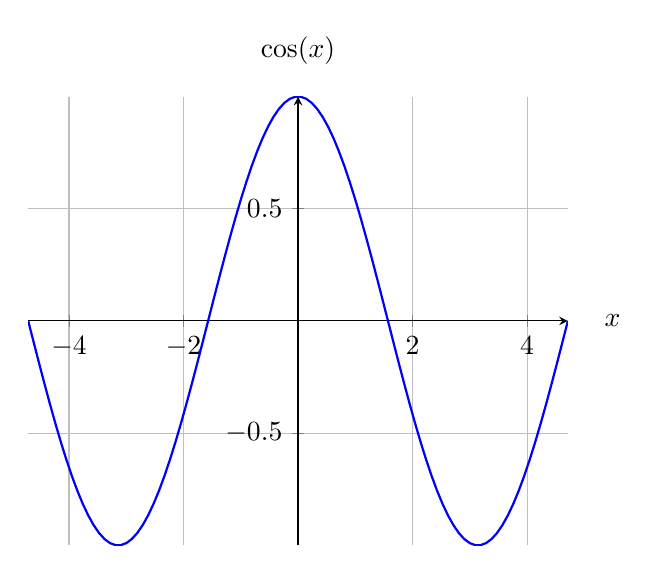
\begin{tikzpicture}
		\begin{axis}[
			xlabel=$x$,
			ylabel=$\cos(x)$,
			domain=-3/2*pi:3/2*pi,
			samples=100,
			axis lines=middle,
			grid=both,
			every axis y label/.style={at={(ticklabel* cs:1.05)}, anchor=south},
			every axis x label/.style={at={(ticklabel* cs:1.05)}, anchor=west},
			]
			\addplot[blue, thick] {cos(deg(x))};
		\end{axis}
	\end{tikzpicture}
	\caption{Cosine function.}
	\label{cos}
\end{figure}

Now we will take a step back and try to achieve the mysterious number for the approximation ratio. Let $\theta_{ij}$ be the angle between $v_{i}$ and $v_{j}$. Then for $\{i,j\} \in E$, its contribution to the objective (in VP) is $\frac{1 - \cos \theta_{ij}}{2}$.

\begin{lemma}[no proof]
	For each $x \in \langle 0, \pi \rangle$ and $\alpha = 0,87856$ it holds that
	
	$$
	\frac{x}{\pi} \geq \alpha \frac{1 - \cos x}{2}
	$$
\end{lemma}

The meaning of it is shown on the picture \ref{meaning}.

\begin{figure}[!ht]\centering
	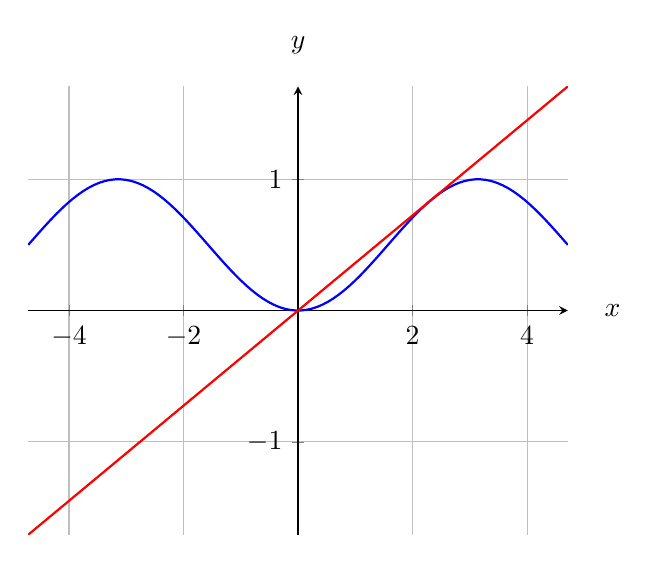
\begin{tikzpicture}
		\begin{axis}[
			xlabel=$x$,
			ylabel=$y$,
			domain=-3/2*pi:3/2*pi,
			samples=100,
			axis lines=middle,
			grid=both,
			every axis y label/.style={at={(ticklabel* cs:1.05)}, anchor=south},
			every axis x label/.style={at={(ticklabel* cs:1.05)}, anchor=west},
			legend pos=outer north east,
			]
			\addplot[blue, thick, label=($(1 - \cos(x)) /2$)] {(1 - cos(deg(x))) / 2};
			\addplot[red, thick, label=($x/(\pi \cdot \alpha)$)] {x / (0.87856 * pi)};
			\legend{}
		\end{axis}
	\end{tikzpicture}
	\caption{The \textcolor{red}{red} function is for $x/(\pi \cdot \alpha)$ and \textcolor{blue}{blue} for $(1 - \cos(x)) /2$.}
	\label{meaning}
\end{figure}

\begin{lemma}
	For $\{i,j\} \in E$ $\Pr [i \text{ and } j \text{ are separated}] = \frac{\theta_{ij}}{\pi}$.
\end{lemma}

\begin{proof}
	Consider the projection of $r$ to the plane defined by $v_i$, $v_j$. Let $W$ be the objective value of our solution:
	
	$$
	\begin{aligned}
		\E [W] & =    & \sum_{\{i,j\} \in E} \frac{\theta_{ij}}{\pi} & \quad \text{(by linearity of expectation)} \\
		       & \geq & \alpha \sum_{\{i,j\} \in E} \frac{1 - \cos (\theta_{ij})}{2} & \quad \text{(by the first lemma)} \\
		       & =    & \alpha \sum_{\{i,j\} \in E} \frac{1 - v_{i}^T v_{j}}{2} & \quad \textbf{(this is our objective functions of VP)} \\
		       & \geq & \alpha \cdot OPT & \quad \text{(because VP is a relaxation)}
	\end{aligned}
	$$
\end{proof}
	\chapter{Edge disjoint path problem}

Some readers may already know what is edge disjoint path problem and also some basic algorithms. But we will have a brief introduction to this topic.

\begin{itemize}
	\item \textbf{INPUT}: $G=(V,E)$ and $(s_{i}, t_{i}) \in V^2$ for all $i \in [k]$.
	\item \textbf{OUTPUT}: $I \subseteq [k]$ and an $s_{i}-t_{i}$ path $P_{i}$ for each $i \in I$, s.t. the selected paths are edge disjoint.
	\item \textbf{OBJECTIVE}: $\max |I|$.
\end{itemize}

It is known that this particular problem is NP-hard. So we will again show some approximation to this problem. \textit{Note: for any fix $k$ it is solvable in polynomial time on undirected graph. But for directed graphs it is NP-hard for $k = 2$.} We will introduce an greedy algorithm that has an parameter.

\begin{algorithm}
	\caption{Greedy algorithm with a catch for parameter $\sqrt{m}$}
	\begin{algorithmic}[1]
		\State $I = \emptyset$
		\While{$\exists i \notin I$ and $\exists s_{i}-t_{i}$ path in $G$, s.t. $|P_{i}| \leq \sqrt{m}$}
			\State $I = I \cup \{i\}$, keep $P_{i}$, $G = G \setminus P_{i}$
		\EndWhile
	\end{algorithmic}
\end{algorithm}

We will denote $OPT$ as the optimal solution of the problem. It will be either a set of paths or set of indexes. Then we will denote $OPT_{S} = \{P \in OPT \mid |P| \leq \sqrt{m}\}$, where the length of a path is set as the number of edges. Then $OPT_{L} = OPT \setminus OPT_{S}$ and $ALG$ as the set given by the algorithm.

Now take the set $OPT_{S} \setminus ALG$. That is path between $s_{i}$ and $t_{i}$ is in this set if there exists $s_{j}-t_{j}$ path obtained by the algorithm which shares an edge. This path has length at most $\sqrt{m}$ and there are $|ALG|$ paths. Thus altogether $|OPT_{S} \setminus ALG| \leq \sqrt{m} |ALG|$.

Next we may see that $|OPT_{L}| \leq \sqrt{m}$, because we have $m$ edges and each one of them is at least $\sqrt{m}$ long. Now we may conclude altogether following result.

$$
|OPT| \leq |OPT_{L}| + |OPT_{S} \setminus ALG| + |ALG| \leq O(\sqrt{m}) |ALG|
$$

Now one can see where the catch in the algorithm is. Consider that there are no such short paths. The algorithm will output no path at all. To fix this we need to change the algorithm such that it will always output at least one path. If there is none then $OPT$ is 0 as well.

\begin{algorithm}
	\caption{Greedy ($\sqrt{m}$)}
	\begin{algorithmic}[1]
		\State $I = \emptyset$
		\While{$\exists i \notin I$ and $\exists s_{i}-t_{i}$ path in $G$, s.t. $|P_{i}| \leq \sqrt{m}$}
		\State $I = I \cup \{i\}$, keep $P_{i}$, $G = G \setminus P_{i}$
		\EndWhile
		\If{\textcolor{Green}{$I = \emptyset$}}
			\State \textcolor{Green}{Connect any $s_{i}-t_{i}$ path if possible.}
		\EndIf
	\end{algorithmic}
\end{algorithm}

Thus we have shown an algorithm that is a $\sqrt{m}$-approximation. Now we consider running the same algorithm but we change the parameter from $\sqrt{m}$ to $n^{2/3}$. Can we obtain $n^{2/3}$-approximation?

\begin{thm}[Khana, Chedari]
	\label{max flow bounded}
	Given an instance of the sum multi-commodity flow problem $G =(V,E)$, \newline $(s_{i}, t_{i}) \in V^2$ for all $i \in [k]$ such that $(\forall i) \ d(s_{i}, t_{i}) \geq l$, then the max multi-commodity flow is $O(\frac{n^2}{l^2})$.
\end{thm}

Before proving this we will show the consequences for our problem. Lets use the algorithm Greedy$(n^{2/3})$. Assume there $\exists P_{i} \in ALG, |P_{i}| \leq n^{2/3}$. Otherwise we use the theorem on the network obtained by $G$ and setting all capacities to one. Then all edges are at least $n^{2/3}$ length so we get the max multi-commodity flow is $O(\frac{n^{2}}{n^{4/3}}) = O(n^{2/3})$. Therefore it means if we choose just one path the approximation ratio will still be $O(n^{2/3})$.

Denote $OPT_{easy} = \{P \in OPT \mid \exists Q \in ALG : Q \cap P \neq \emptyset\}$. With this we know that $|OPT_{easy}| \leq n^{2/3} |ALG|$ by the same argument as it was already mentioned before.

We will look at $\forall (s_{i}, t_{i}) \in (OPT \setminus OPT_{easy}) \setminus ALG$. What can we say about such $d(s_{i}, t_{i})$ at the end of the loop of the algorithm. Clearly because it was not chosen either there is some intersection with another path, but this is remove by $OPT_{easy}$, so the other option is only that $d(s_{i}, t_{i}) > n^{2/3}$. Hence $|(OPT \setminus OPT_{easy}) \setminus ALG| \leq O(n^{2/3})$ by the theorem and the same argument which was already mentioned. Altogether we have:

$$
|OPT| \leq |OPT_{easy}| + |(OPT \setminus OPT_{easy}) \setminus ALG| + |ALG| = O(n^{2/3}) |ALG|
$$

Now we only need to prove the theorem since it is the base of our arguments for obtaining $O(n^{2/3})$-approximation algorithm.

\begin{proof}
	We will split the vertices into two sets:
	
	\begin{enumerate}
		\item \textbf{low degree vertex} is when $\deg(v) \leq \frac{6 n}{l}$
		\item \textbf{high degree vertex} is when $\deg(v) > \frac{6 n}{l}$
	\end{enumerate}
	
	Also we will assume $l$ is a multiple of 6. Otherwise it get lost in the $O$ notation. To finish the proof we will use an observation.
	
	\begin{observ}
		Any $s_{i}-t_{i}$ path (denote it as $s-t$) uses at least $l/6$ low degree vertices.
	\end{observ}
	
	\begin{proof}[Proof of observation]
		Consider running BFS on the graph starting from $s$. We denote $L_{i} = \{u \in V : d(s,u) = i\}$. Note that edges are only within one layer or only between adjacent layers. Let $B_{i}$ be a block of three consecutive layers $\{L_{3i}, L_{3i+1}, L_{3i+2}\}$. Because the length to $t$ is at least $l$ then there is at least $l/3$ blocks. Assume that $< l/6$ layers consists of only low degree vertices. Otherwise the observation obviously holds. Now discard all blocks containing a layer of only low degree vertices. As there are $\geq l/3$ blocks at least $\geq l/6$ blocks remain. Then the smallest remaining block is of size $\leq \frac{n}{l/6} = 6n/l$ which can be seen by pigeonhole principle. For the vertices in the middle layer we know all neighbors are within the block. Therefore it is a low degree vertex. This is a contradiction because we still have a block having one layer with low degree vertices only.
	\end{proof}
	
	Now for the theorem we know a \textbf{unit} of flow between any pair $s_{i}-t_{i}$ consumes $\mathbf{\Omega(l)}$ cpacity of edges adjacent to low degree vertices. And the total capacity adjacent to low degree vertices is $\leq n \deg(v) \leq n (6n/l) = O(n^2/l)$. Which gives us $O(n^2/l^2)$.
\end{proof}

This is an example of greedy algorithm and the fact that using it with different parameter may result in better approximation, but the analysis is way harder. We also saw using flows to limit paths, but this has also its limits. We will show a counterexample a graph called \textbf{Brick wall}.

\begin{figure}[!ht]\centering
	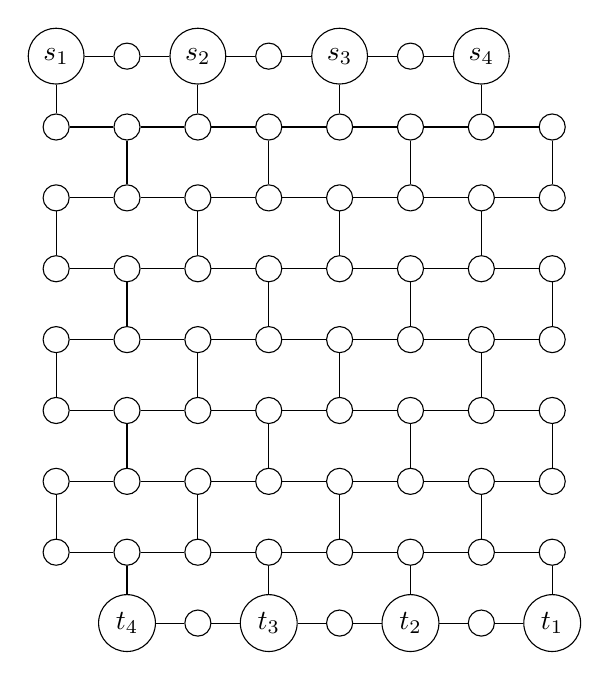
\begin{tikzpicture}[node distance={9mm}, main/.style = {draw, circle}]
		\node[main] (0) {$s_{1}$};
		\node[main] (1) [right of=0] {};
		\draw (0) -- (1);
		\node[main] (2) [right of=1] {$s_{2}$};
		\draw (1) -- (2);
		\node[main] (3) [right of=2] {};
		\draw (2) -- (3);
		\node[main] (4) [right of=3] {$s_{3}$};
		\draw (3) -- (4);
		\node[main] (5) [right of=4] {};
		\draw (4) -- (5);
		\node[main] (6) [right of=5] {$s_{4}$};
		\draw (5) -- (6);
		\node[main] (10) [below of=0] {};
		\draw (10) -- (0);
		\node[main] (11) [right of=10] {};
		\draw (11) -- (10);
		\node[main] (12) [right of=11] {};
		\draw (12) -- (11);
		\draw (12) -- (2);
		\node[main] (13) [right of=12] {};
		\draw (13) -- (12);
		\node[main] (14) [right of=13] {};
		\draw (14) -- (13);
		\draw (14) -- (4);
		\node[main] (15) [right of=14] {};
		\draw (15) -- (14);
		\node[main] (16) [right of=15] {};
		\draw (16) -- (15);
		\draw (16) -- (6);
		\node[main] (17) [right of=16] {};
		\draw (17) -- (16);
		\node[main] (20) [below of=10] {};
		\node[main] (21) [right of=20] {};
		\draw (21) -- (20);
		\draw (21) -- (11);
		\node[main] (22) [right of=21] {};
		\draw (22) -- (21);
		\node[main] (23) [right of=22] {};
		\draw (23) -- (22);
		\draw (23) -- (13);
		\node[main] (24) [right of=23] {};
		\draw (24) -- (23);
		\node[main] (25) [right of=24] {};
		\draw (25) -- (24);
		\draw (25) -- (15);
		\node[main] (26) [right of=25] {};
		\draw (26) -- (25);
		\node[main] (27) [right of=26] {};
		\draw (27) -- (26);
		\draw (27) -- (17);
		\node[main] (30) [below of=20] {};
		\draw (30) -- (20);
		\node[main] (31) [right of=30] {};
		\draw (31) -- (30);
		\node[main] (32) [right of=31] {};
		\draw (32) -- (31);
		\draw (32) -- (22);
		\node[main] (33) [right of=32] {};
		\draw (33) -- (32);
		\node[main] (34) [right of=33] {};
		\draw (34) -- (33);
		\draw (34) -- (24);
		\node[main] (35) [right of=34] {};
		\draw (35) -- (34);
		\node[main] (36) [right of=35] {};
		\draw (36) -- (35);
		\draw (36) -- (26);
		\node[main] (37) [right of=36] {};
		\draw (37) -- (36);
		\node[main] (40) [below of=30] {};
		\node[main] (41) [right of=40] {};
		\draw (41) -- (40);
		\draw (41) -- (31);
		\node[main] (42) [right of=41] {};
		\draw (42) -- (41);
		\node[main] (43) [right of=42] {};
		\draw (43) -- (42);
		\draw (43) -- (33);
		\node[main] (44) [right of=43] {};
		\draw (44) -- (43);
		\node[main] (45) [right of=44] {};
		\draw (45) -- (44);
		\draw (45) -- (35);
		\node[main] (46) [right of=45] {};
		\draw (46) -- (45);
		\node[main] (47) [right of=46] {};
		\draw (47) -- (46);
		\draw (47) -- (37);
		\node[main] (50) [below of=40] {};
		\draw (50) -- (40);
		\node[main] (51) [right of=50] {};
		\draw (51) -- (50);
		\node[main] (52) [right of=51] {};
		\draw (52) -- (51);
		\draw (52) -- (42);
		\node[main] (53) [right of=52] {};
		\draw (53) -- (52);
		\node[main] (54) [right of=53] {};
		\draw (54) -- (53);
		\draw (54) -- (44);
		\node[main] (55) [right of=54] {};
		\draw (55) -- (54);
		\node[main] (56) [right of=55] {};
		\draw (56) -- (55);
		\draw (56) -- (46);
		\node[main] (57) [right of=56] {};
		\draw (57) -- (56);
		\node[main] (60) [below of=50] {};
		\node[main] (61) [right of=60] {};
		\draw (61) -- (60);
		\draw (61) -- (51);
		\node[main] (62) [right of=61] {};
		\draw (62) -- (61);
		\node[main] (63) [right of=62] {};
		\draw (63) -- (62);
		\draw (63) -- (53);
		\node[main] (64) [right of=63] {};
		\draw (64) -- (63);
		\node[main] (65) [right of=64] {};
		\draw (65) -- (64);
		\draw (65) -- (55);
		\node[main] (66) [right of=65] {};
		\draw (66) -- (65);
		\node[main] (67) [right of=66] {};
		\draw (67) -- (66);
		\draw (67) -- (57);
		\node[main] (70) [below of=60] {};
		\draw (70) -- (60);
		\node[main] (71) [right of=70] {};
		\draw (71) -- (70);
		\node[main] (72) [right of=71] {};
		\draw (72) -- (71);
		\draw (72) -- (62);
		\node[main] (73) [right of=72] {};
		\draw (73) -- (72);
		\node[main] (74) [right of=73] {};
		\draw (74) -- (73);
		\draw (74) -- (64);
		\node[main] (75) [right of=74] {};
		\draw (75) -- (74);
		\node[main] (76) [right of=75] {};
		\draw (76) -- (75);
		\draw (76) -- (66);
		\node[main] (77) [right of=76] {};
		\draw (77) -- (76);
		\node[main] (81) [below of=71] {$t_{4}$};
		\node[main] (82) [right of=81] {};
		\draw (81) -- (71);
		\draw (82) -- (81);
		\node[main] (83) [right of=82] {$t_{3}$};
		\draw (83) -- (82);
		\node[main] (84) [right of=83] {};
		\draw (83) -- (73);
		\draw (84) -- (83);
		\node[main] (85) [right of=84] {$t_{2}$};
		\draw (85) -- (84);
		\node[main] (86) [right of=85] {};
		\draw (85) -- (75);
		\draw (86) -- (85);
		\node[main] (87) [right of=86] {$t_{1}$};
		\draw (77) -- (87);
		\draw (87) -- (86);
	\end{tikzpicture}
	\caption{Example of a \textbf{brick wall} graph for $k = 4$.}
	\label{brick-wall}
\end{figure}

The graph you may see at the picture \ref{brick-wall} is planar. Also it can be generalized to $k$ where there are $k$ pairs of bricks underneath. The edge disjoint problem optimum is 1, which we can see on picture \ref{edg}. And the max multi flow optimum is at least $k/2 = O(\sqrt{n})$, which can be seen on picture \ref{max-flow}.


\begin{figure}[!ht]\centering
	\begin{subfigure}{0.45\textwidth}\centering
		\begin{tikzpicture}[node distance={9mm}, main/.style = {draw, circle}]
			\node[main] (0) {$s_{1}$};
			\node[main] (1) [right of=0] {};
			\draw (0) -- (1);
			\node[main] (2) [right of=1] {$s_{2}$};
			\draw (1) -- (2);
			\node[main] (3) [right of=2] {};
			\draw (2) -- (3);
			\node[main] (4) [right of=3] {$s_{3}$};
			\draw (3) -- (4);
			\node[main] (5) [right of=4] {};
			\draw (4) -- (5);
			\node[main] (6) [right of=5] {$s_{4}$};
			\draw (5) -- (6);
			\node[main] (10) [below of=0] {};
			\draw (10) -- (0);
			\node[main] (11) [right of=10] {};
			\draw (11) -- (10);
			\node[main] (12) [right of=11] {};
			\draw (12) -- (11);
			\draw (12) -- (2);
			\node[main] (13) [right of=12] {};
			\draw (13) -- (12);
			\node[main] (14) [right of=13] {};
			\draw (14) -- (13);
			\draw (14) -- (4);
			\node[main] (15) [right of=14] {};
			\draw (15) -- (14);
			\node[main] (16) [right of=15] {};
			\draw (16) -- (15);
			\draw (16) -- (6);
			\node[main] (17) [right of=16] {};
			\draw (17) -- (16);
			\node[main] (20) [below of=10] {};
			\node[main] (21) [right of=20] {};
			\draw (21) -- (20);
			\draw (21) -- (11);
			\node[main] (22) [right of=21] {};
			\draw (22) -- (21);
			\node[main] (23) [right of=22] {};
			\draw (23) -- (22);
			\draw (23) -- (13);
			\node[main] (24) [right of=23] {};
			\draw (24) -- (23);
			\node[main] (25) [right of=24] {};
			\draw (25) -- (24);
			\draw (25) -- (15);
			\node[main] (26) [right of=25] {};
			\draw (26) -- (25);
			\node[main] (27) [right of=26] {};
			\draw (27) -- (26);
			\draw (27) -- (17);
			\node[main] (30) [below of=20] {};
			\draw (30) -- (20);
			\node[main] (31) [right of=30] {};
			\draw (31) -- (30);
			\node[main] (32) [right of=31] {};
			\draw (32) -- (31);
			\draw (32) -- (22);
			\node[main] (33) [right of=32] {};
			\draw (33) -- (32);
			\node[main] (34) [right of=33] {};
			\draw (34) -- (33);
			\draw (34) -- (24);
			\node[main] (35) [right of=34] {};
			\draw (35) -- (34);
			\node[main] (36) [right of=35] {};
			\draw (36) -- (35);
			\draw (36) -- (26);
			\node[main] (37) [right of=36] {};
			\draw (37) -- (36);
			\node[main] (40) [below of=30] {};
			\node[main] (41) [right of=40] {};
			\draw (41) -- (40);
			\draw (41) -- (31);
			\node[main] (42) [right of=41] {};
			\draw (42) -- (41);
			\node[main] (43) [right of=42] {};
			\draw (43) -- (42);
			\draw (43) -- (33);
			\node[main] (44) [right of=43] {};
			\draw (44) -- (43);
			\node[main] (45) [right of=44] {};
			\draw (45) -- (44);
			\draw (45) -- (35);
			\node[main] (46) [right of=45] {};
			\draw (46) -- (45);
			\node[main] (47) [right of=46] {};
			\draw (47) -- (46);
			\draw (47) -- (37);
			\node[main] (50) [below of=40] {};
			\draw (50) -- (40);
			\node[main] (51) [right of=50] {};
			\draw (51) -- (50);
			\node[main] (52) [right of=51] {};
			\draw (52) -- (51);
			\draw (52) -- (42);
			\node[main] (53) [right of=52] {};
			\draw (53) -- (52);
			\node[main] (54) [right of=53] {};
			\draw (54) -- (53);
			\draw (54) -- (44);
			\node[main] (55) [right of=54] {};
			\draw (55) -- (54);
			\node[main] (56) [right of=55] {};
			\draw (56) -- (55);
			\draw (56) -- (46);
			\node[main] (57) [right of=56] {};
			\draw (57) -- (56);
			\node[main] (60) [below of=50] {};
			\node[main] (61) [right of=60] {};
			\draw (61) -- (60);
			\draw (61) -- (51);
			\node[main] (62) [right of=61] {};
			\draw (62) -- (61);
			\node[main] (63) [right of=62] {};
			\draw (63) -- (62);
			\draw (63) -- (53);
			\node[main] (64) [right of=63] {};
			\draw (64) -- (63);
			\node[main] (65) [right of=64] {};
			\draw (65) -- (64);
			\draw (65) -- (55);
			\node[main] (66) [right of=65] {};
			\draw (66) -- (65);
			\node[main] (67) [right of=66] {};
			\draw (67) -- (66);
			\draw (67) -- (57);
			\node[main] (70) [below of=60] {};
			\draw (70) -- (60);
			\node[main] (71) [right of=70] {};
			\draw (71) -- (70);
			\node[main] (72) [right of=71] {};
			\draw (72) -- (71);
			\draw (72) -- (62);
			\node[main] (73) [right of=72] {};
			\draw (73) -- (72);
			\node[main] (74) [right of=73] {};
			\draw (74) -- (73);
			\draw (74) -- (64);
			\node[main] (75) [right of=74] {};
			\draw (75) -- (74);
			\node[main] (76) [right of=75] {};
			\draw (76) -- (75);
			\draw (76) -- (66);
			\node[main] (77) [right of=76] {};
			\draw (77) -- (76);
			\node[main] (81) [below of=71] {$t_{4}$};
			\node[main] (82) [right of=81] {};
			\draw (81) -- (71);
			\draw (82) -- (81);
			\node[main] (83) [right of=82] {$t_{3}$};
			\draw (77) -- (87);
			\draw (83) -- (82);
			\node[main] (84) [right of=83] {};
			\draw (83) -- (73);
			\draw (84) -- (83);
			\node[main] (85) [right of=84] {$t_{2}$};
			\draw (77) -- (87);
			\draw (85) -- (84);
			\node[main] (86) [right of=85] {};
			\draw (85) -- (75);
			\draw (86) -- (85);
			\node[main] (87) [right of=86] {$t_{1}$};
			\draw (77) -- (87);
			\draw (87) -- (86);
			\path[color=blue, line width = 4] (0) edge (10)
			(10) edge (11)
			(11) edge (21)
			(21) edge (22)
			(22) edge (32)
			(32) edge (33)
			(33) edge (43)
			(43) edge (44)
			(44) edge (54)
			(54) edge (55)
			(55) edge (65)
			(65) edge (66)
			(66) edge (76)
			(76) edge (77)
			(77) edge (87);
		\end{tikzpicture}
		\caption{Edge disjoint problem.}
		\label{edg}
	\end{subfigure}\centering
	\begin{subfigure}{0.45\textwidth}\centering
		\begin{tikzpicture}[node distance={9mm}, main/.style = {draw, circle}]
			\node[main] (0) {$s_{1}$};
			\node[main] (1) [right of=0] {};
			\draw (0) -- (1);
			\node[main] (2) [right of=1] {$s_{2}$};
			\draw (1) -- (2);
			\node[main] (3) [right of=2] {};
			\draw (2) -- (3);
			\node[main] (4) [right of=3] {$s_{3}$};
			\draw (3) -- (4);
			\node[main] (5) [right of=4] {};
			\draw (4) -- (5);
			\node[main] (6) [right of=5] {$s_{4}$};
			\draw (5) -- (6);
			\node[main] (10) [below of=0] {};
			\draw (10) -- (0);
			\node[main] (11) [right of=10] {};
			\draw (11) -- (10);
			\node[main] (12) [right of=11] {};
			\draw (12) -- (11);
			\draw (12) -- (2);
			\node[main] (13) [right of=12] {};
			\draw (13) -- (12);
			\node[main] (14) [right of=13] {};
			\draw (14) -- (13);
			\draw (14) -- (4);
			\node[main] (15) [right of=14] {};
			\draw (15) -- (14);
			\node[main] (16) [right of=15] {};
			\draw (16) -- (15);
			\draw (16) -- (6);
			\node[main] (17) [right of=16] {};
			\draw (17) -- (16);
			\node[main] (20) [below of=10] {};
			\node[main] (21) [right of=20] {};
			\draw (21) -- (20);
			\draw (21) -- (11);
			\node[main] (22) [right of=21] {};
			\draw (22) -- (21);
			\node[main] (23) [right of=22] {};
			\draw (23) -- (22);
			\draw (23) -- (13);
			\node[main] (24) [right of=23] {};
			\draw (24) -- (23);
			\node[main] (25) [right of=24] {};
			\draw (25) -- (24);
			\draw (25) -- (15);
			\node[main] (26) [right of=25] {};
			\draw (26) -- (25);
			\node[main] (27) [right of=26] {};
			\draw (27) -- (26);
			\draw (27) -- (17);
			\node[main] (30) [below of=20] {};
			\draw (30) -- (20);
			\node[main] (31) [right of=30] {};
			\draw (31) -- (30);
			\node[main] (32) [right of=31] {};
			\draw (32) -- (31);
			\draw (32) -- (22);
			\node[main] (33) [right of=32] {};
			\draw (33) -- (32);
			\node[main] (34) [right of=33] {};
			\draw (34) -- (33);
			\draw (34) -- (24);
			\node[main] (35) [right of=34] {};
			\draw (35) -- (34);
			\node[main] (36) [right of=35] {};
			\draw (36) -- (35);
			\draw (36) -- (26);
			\node[main] (37) [right of=36] {};
			\draw (37) -- (36);
			\node[main] (40) [below of=30] {};
			\node[main] (41) [right of=40] {};
			\draw (41) -- (40);
			\draw (41) -- (31);
			\node[main] (42) [right of=41] {};
			\draw (42) -- (41);
			\node[main] (43) [right of=42] {};
			\draw (43) -- (42);
			\draw (43) -- (33);
			\node[main] (44) [right of=43] {};
			\draw (44) -- (43);
			\node[main] (45) [right of=44] {};
			\draw (45) -- (44);
			\draw (45) -- (35);
			\node[main] (46) [right of=45] {};
			\draw (46) -- (45);
			\node[main] (47) [right of=46] {};
			\draw (47) -- (46);
			\draw (47) -- (37);
			\node[main] (50) [below of=40] {};
			\draw (50) -- (40);
			\node[main] (51) [right of=50] {};
			\draw (51) -- (50);
			\node[main] (52) [right of=51] {};
			\draw (52) -- (51);
			\draw (52) -- (42);
			\node[main] (53) [right of=52] {};
			\draw (53) -- (52);
			\node[main] (54) [right of=53] {};
			\draw (54) -- (53);
			\draw (54) -- (44);
			\node[main] (55) [right of=54] {};
			\draw (55) -- (54);
			\node[main] (56) [right of=55] {};
			\draw (56) -- (55);
			\draw (56) -- (46);
			\node[main] (57) [right of=56] {};
			\draw (57) -- (56);
			\node[main] (60) [below of=50] {};
			\node[main] (61) [right of=60] {};
			\draw (61) -- (60);
			\draw (61) -- (51);
			\node[main] (62) [right of=61] {};
			\draw (62) -- (61);
			\node[main] (63) [right of=62] {};
			\draw (63) -- (62);
			\draw (63) -- (53);
			\node[main] (64) [right of=63] {};
			\draw (64) -- (63);
			\node[main] (65) [right of=64] {};
			\draw (65) -- (64);
			\draw (65) -- (55);
			\node[main] (66) [right of=65] {};
			\draw (66) -- (65);
			\node[main] (67) [right of=66] {};
			\draw (67) -- (66);
			\draw (67) -- (57);
			\node[main] (70) [below of=60] {};
			\draw (70) -- (60);
			\node[main] (71) [right of=70] {};
			\draw (71) -- (70);
			\node[main] (72) [right of=71] {};
			\draw (72) -- (71);
			\draw (72) -- (62);
			\node[main] (73) [right of=72] {};
			\draw (73) -- (72);
			\node[main] (74) [right of=73] {};
			\draw (74) -- (73);
			\draw (74) -- (64);
			\node[main] (75) [right of=74] {};
			\draw (75) -- (74);
			\node[main] (76) [right of=75] {};
			\draw (76) -- (75);
			\draw (76) -- (66);
			\node[main] (77) [right of=76] {};
			\draw (77) -- (76);
			\node[main] (81) [below of=71] {$t_{4}$};
			\node[main] (82) [right of=81] {};
			\draw (81) -- (71);
			\draw (82) -- (81);
			\node[main] (83) [right of=82] {$t_{3}$};
			\draw (77) -- (87);
			\draw (83) -- (82);
			\node[main] (84) [right of=83] {};
			\draw (83) -- (73);
			\draw (84) -- (83);
			\node[main] (85) [right of=84] {$t_{2}$};
			\draw (77) -- (87);
			\draw (85) -- (84);
			\node[main] (86) [right of=85] {};
			\draw (85) -- (75);
			\draw (86) -- (85);
			\node[main] (87) [right of=86] {$t_{1}$};
			\draw (77) -- (87);
			\draw (87) -- (86);
			\path[color=orange, line width = 4] (0) edge (10)
			(10) edge (11)
			(11) edge (21)
			(21) edge (22)
			(22) edge (32)
			(32) edge (33)
			(33) edge (43)
			(43) edge (44)
			(44) edge (54)
			(54) edge (55)
			(55) edge (65)
			(65) edge (66)
			(66) edge (76)
			(76) edge (77)
			(77) edge (87);
			\path[color=VioletRed, line width = 4] (2) edge (12)
			(12) edge (13)
			(13) edge (23)
			(23) edge (24)
			(24) edge (34)
			(34) edge (35)
			(35) edge (45)
			(45) edge (46)
			(46) edge (56)
			(56) edge (57)
			(57) edge (67)
			(67) edge (66)
			(66) edge (65)
			(65) edge (64)
			(64) edge (74)	(74) edge (75)	(75) edge (85);
			\path[color=blue, line width = 4] (4) edge (14)
			(14) edge (15)
			(15) edge (25)
			(25) edge (26)
			(26) edge (36)
			(36) edge (37)
			(37) edge (47)
			(47) edge (46)
			(46) edge (45)
			(45) edge (44)
			(44) edge (43)
			(43) edge (42)
			(42) edge (52)
			(52) edge (53)	(53) edge (63)	(63) edge (62)	(62) edge (72)	(72) edge (73)	(73) edge (83);
			\path[color=Green, line width = 4] (6) edge (16)
			(16) edge (17)
			(17) edge (27)
			(27) edge (26)
			(26) edge (25)
			(25) edge (24)
			(24) edge (23)
			(23) edge (22)
			(22) edge (21)
			(21) edge (20)
			(20) edge (30)
			(30) edge (31)	(31) edge (41)	(41) edge (40)	(40) edge (50)
			(50) edge (51)	(51) edge (61)	(61) edge (60)	(60) edge (70)	(70) edge (71)	(71) edge (81);
		\end{tikzpicture}
		\caption{Max multi flow; paths have $1/2$.}
		\label{max-flow}
	\end{subfigure}
	\caption{Example of optimalization problems.}
\end{figure}

\section{Edge disjoint path problem and flow number}

We will be again considering undirected graph $G=(V,E)$. And also a concurrent multi-commodity flow problem (or CMFP for short) with $(s_{i}, t_{i})$ commodities for $i = 1, \dots, k$ and their demands $d_{i} \in \R^{+}$. We will denote $S$ as a feasible solution for such problem.

\begin{defn}
	\textbf{Flow value} is the value of the objective function for $S$.
\end{defn}

\begin{defn}
	\textbf{Balanced instance} of the CMFP such that
	
	$$
	\forall v \in V(G) : \sum_{i: s_{i} = v} d_{i} = \deg(v) = \sum_{i: t_{i} = v} d_{i}.
	$$
\end{defn}

It may also be defined with inequalities. We will be calling this \textbf{balanced multi-commodity flow problem} (or BMFP for short).

\begin{defn}
	\textbf{Product multi-commodity flow} (PMFP for short) is an instance where
	
	\begin{itemize}
		\item There is a value $\pi(v) \in \R^+$ associated with every vertex $v \in V$.
		\item There is a commodity for every ordered pair of vertices $(u,v)$ of demand $\pi(u) \cdot \pi(v)$.
	\end{itemize}
\end{defn}

\begin{defn}
	\textbf{Dilation}$(S)$ denoted as $D(S)$ is the length of the longest path in $S$.
\end{defn}

\begin{defn}
	\textbf{Congestion}$(S)$ denoted as $C(S)$ is the inverse of the flow value in $S$.
\end{defn}

As a side-note when there was a problem for a networks in a computers to find best paths for sending packets it can be shown that the upper bound for the time is somewhat connected to similiar terms, particularly $O(C + D)$.

Now for a given $G = (V,E)$ we denote $I_{0}$ as an instance of the PMFP with $\pi(u) = \frac{\deg(u)}{\sqrt{2|E|}}$. \textit{Note that $2|E| = \sum_{v \in V} \deg(v)$.}

\begin{defn}
	\textbf{Flow number} of a graph $G$ denoted as $F(G)$ is
	
	$$
	\min_{\text{feasible solution } S \text{ for } I_{0}} \{ \max \{ C(S), D(S) \} \}
	$$
\end{defn}

\begin{claim}
	There is a polynomial time algorithm that computes $F(G)$ for every graph $G$.
\end{claim}

\begin{proof}
	Lets assume $V = \{v_{1}, v_{2}, \dots, v_{n}\}$. For $L \in \N$ we define graph $G_{L} = (V', E')$. This is a layered graph with $L+1$ layers. To be precise it is defined as follows
	
	$$
	\begin{aligned}
		V_{i} &= \{v_{i1}, v_{i2}, \dots, v_{in}\}, &\quad \forall i \in 0, 1, \dots, L \\
		E_{i} &= \{(v_{(i-1)j}, v_{ik}) \mid \{v_{j}, v_{k}\} \in E \} \cup \{(v_{(i-1)j}, v_{ij}) \mid v_{j} \in V\}, &\quad \forall i \in 1,2, \dots, L \\
	\end{aligned}
	$$
	
	$$
	\text{then } V' = \bigcup_{i = 0}^{L} V_{i} \text{ and } E' = \bigcup_{i=1}^{L} E_{i}.
	$$
	
	Note that we do not keep $V$ and $E$ from the original graph.
	
	Now consider the following instance of CMFP. $\forall (v_{i}, v_{j}) \in V^2$ we set commodity between $v_{0i}$ and $v_{Lj}$ of demand $\pi(v_{i}) \cdot \pi(v_{j})$ (where $\pi$ is taken from $I_{0}$). We also define a special request. $\forall \{v_{i}, v_{j}\} \in E$ the sum of flows over all edges in
	
	$$
	\bigcup_{k = 1}^{L} \{ (v_{(k-1)i}, v_{kj}), (v_{(k-1)j}, v_{ki}) \}
	$$
	
	has to be at most 1. This is just a linear constrained so we are able to solve this in polynomial time. With this requirement we are able to map the solution to the original graph $G$. Also the dilation is $L$ and to compute the congestion is easy to do from the result of LP. In other words $\forall L \in \{1, \dots, |V|\}$ find opt of this LP in $G_{L}$ and denote it as $S_{L}$. Then let $S_{L}'$ be the corresponding flow in $G$. Hence the following holds.
	
	$$
	F(G) = \min_{L = 1, \dots, |V|} \{ \max \{ C(S_{L}'), D(S_{L}')\} \}
	$$
\end{proof}

\begin{figure}[!ht]\centering
	\begin{subfigure}{0.45\textwidth}\centering
		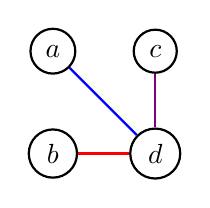
\begin{tikzpicture}[node distance={13mm}, main/.style = {draw, thick, circle}]
			\node[main] (a) [] {$a$};
			\node[main] (b) [below of=a] {$b$};
			\node[main] (c) [right of=a] {$c$};
			\node[main] (d) [right of=b] {$d$};
			\draw[color=blue, thick] (a) edge (d);
			\draw[color=red, thick] (b) edge (d);
			\draw[color=violet, thick] (c) edge (d);
		\end{tikzpicture}
		\caption{Original graph $G$.}
	\end{subfigure}
	\begin{subfigure}{0.45\textwidth}\centering
		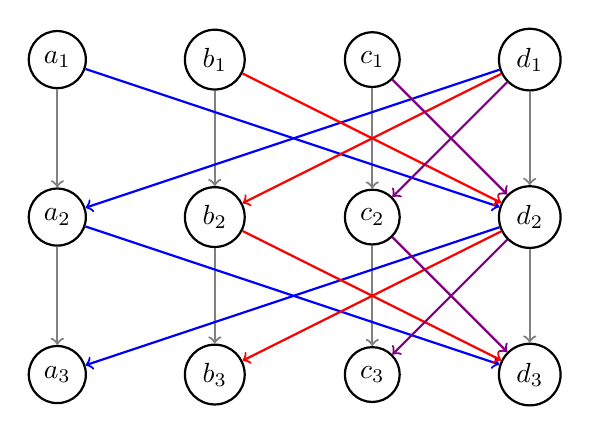
\begin{tikzpicture}[node distance={20mm}, main/.style = {draw, thick, circle}]
			\node[main] (a1) [] {$a_{1}$};
			\node[main] (b1) [right of=a1] {$b_{1}$};
			\node[main] (c1) [right of=b1] {$c_{1}$};
			\node[main] (d1) [right of=c1] {$d_{1}$};
			
			\node[main] (a2) [below of=a1] {$a_{2}$};
			\node[main] (b2) [right of=a2] {$b_{2}$};
			\node[main] (c2) [right of=b2] {$c_{2}$};
			\node[main] (d2) [right of=c2] {$d_{2}$};
			
			\node[main] (a3) [below of=a2] {$a_{3}$};
			\node[main] (b3) [right of=a3] {$b_{3}$};
			\node[main] (c3) [right of=b3] {$c_{3}$};
			\node[main] (d3) [right of=c3] {$d_{3}$};
			
			\path[->, color=gray, thick] (a1) edge (a2) (a2) edge (a3);
			\path[->, color=gray, thick] (b1) edge (b2) (b2) edge (b3);
			\path[->, color=gray, thick] (c1) edge (c2) (c2) edge (c3);
			\path[->, color=gray, thick] (d1) edge (d2) (d2) edge (d3);
			
			\path[->, color=blue, thick] (a1) edge (d2) (d1) edge (a2)
			                             (a2) edge (d3) (d2) edge (a3);
			                               
			\path[->, color=red, thick] (b1) edge (d2) (d1) edge (b2)
			                            (b2) edge (d3) (d2) edge (b3);
			
			\path[->, color=violet, thick] (c1) edge (d2) (d1) edge (c2)
			                               (c2) edge (d3) (d2) edge (c3);
			
		\end{tikzpicture}
		\caption{Layered graph $G_{L}$ for $L = 3$.}
	\end{subfigure}
	\caption{Shown a visualization of a graph $G$ and its layered version $G_{L}$.}
\end{figure}

\begin{claim}
	For any graph $G$ with flow number $F = F(G)$ and an instance $I$ of the BMFP in $G$, there is a feasible solution for $I$ with congestion and dilation at most $2F$.
\end{claim}

\begin{proof}
	For every $(s_{i}, t_{i}) \in I$ we define two instances:
	
	$$
	\begin{aligned}
		I_{1} &: \forall u \in V \text{ add commodity } (s_{i}, u) \text{ of demand } \frac{d_{i} \deg(u)}{2|E|} \\
		I_{2} &: \forall u \in V \text{ add commodity } (u, t_{i}) \text{ of demand } \frac{d_{i} \deg(u)}{2|E|} \\
	\end{aligned}
	$$
	
	Note that $\sum_{v \in V} \frac{d_{i} \deg(v)}{2|E|} = d_{i}$. For $v,w$ what is the sum of demands between $v$ and $w$ in $I_{1}$?
	
	$$
	\sum_{i: s_{i} = v} \frac{d_{i} \deg(w)}{2|E|} = \frac{\deg(w)}{2|E|} \sum_{i: s_{i} = v} d_{i} = \frac{\deg(w)}{2|E|} \deg(v) = \frac{\deg(w) \deg(v)}{2|E|}
	$$
	
	This means that $I_{1}$ is actually $I_{0}$. Similarly it can be shown that $I_{2} = I_{0}$. Hence the $F$ will be doubled for both $I_{1}$ and $I_{2}$ thus getting at most $2F$.
\end{proof}

\begin{lemma}[Flow shortening]
	Let $G = (V,E)$ be a graph and $F = F(G)$ be its flow number. For any $\epsilon \in [0,1]$ and any feasible flow $S$ in $G$ of flow value $f$, for an instance of CMFP. There exists a feasible flow of flow value $\geq \frac{f}{1+\epsilon}$ that uses paths of lengths $\leq 2F(1+\frac{1}{\epsilon})$.
\end{lemma}

Before we properly show the proof we show the idea behind it. We set $L = \frac{2F}{\epsilon}$ and for every path we find the first $L$ vertices and last $L$ vertices. In some paths they may overlap. We will connect the opposite vertices and scale demands and flows, so it will eventually work.

\begin{proof}
	Denote $\mathcal{O}$ the set of the paths in $S$. For $p \in \mathcal{O}$ denote $f_{p}$ as the amount of flow on path $p$. Now let $\mathcal{O}' = \{p \in \mathcal{O} \mid |p| > L\}$ for $L = \frac{2F}{\epsilon}$. For a path $p \in \mathcal{O}'$ let $a_{p,1}, \dots, a_{p,L}$ be the \textcolor{violet}{first} $L$ vertices on path $p$. And let $b_{p,L}, \dots, b_{p,1}$ be the \textcolor{orange}{last} $L$ vertices on path $p$. (As you may see on picture \ref{shortening-path}). Now we define
	
	\begin{figure}[!ht]\centering
		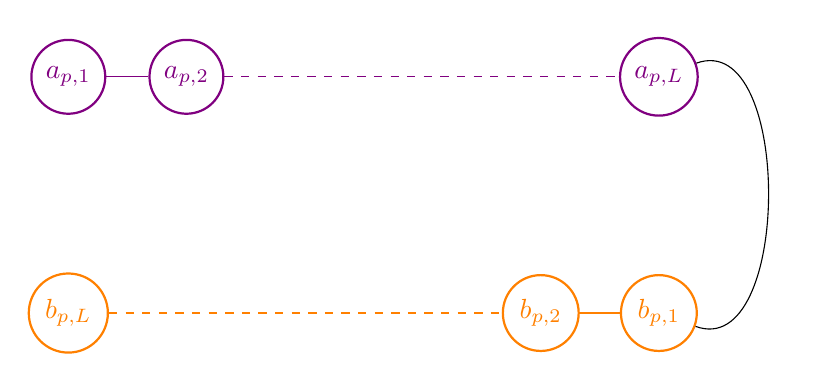
\begin{tikzpicture}[node distance={15mm}, main/.style = {draw, thick, circle}]
			\node[main, color=violet] (1) {$a_{p,1}$};
			\node[below of = 1] (phantom) {};
			\node[main, right of = 1, color=violet] (2) {$a_{p,2}$};
			\node[right of = 2] (3) {};
			\node[right of = 3] (4) {};
			\node[right of = 4] (5) {};
			\node[main, right of = 5, color=violet] (6) {$a_{p,L}$};
			\node[main, below of = phantom, color=orange] (7) {$b_{p,L}$};
			\node[right of = 7] (8) {};
			\node[right of = 8] (9) {};
			\node[right of = 9] (10) {};
			\node[main, right of = 10, color=orange] (11) {$b_{p,2}$};
			\node[main, right of = 11, color=orange] (12) {$b_{p,1}$};
			\draw[color=violet] (1) edge (2);
			\draw[color=orange] (12) edge (11);
			\draw[color=violet, dashed] (2) edge (6);
			\draw[color=orange, dashed] (7) edge (11);
			\draw[color=black, bend right = 110] (12) edge (6);
		\end{tikzpicture}
		\caption{Illustration of the point in the path $p$.}
		\label{shortening-path}
	\end{figure}
	
	$$
	\mathcal{U} = \bigcup_{p \in \mathcal{O}'} \bigcup_{i = 1}^{L} (a_{p,i}, b_{p,i}, f_{p})
	$$
	
	which will be a new instance CMFP with demands $f_{p}$. Also denote $\mathcal{P}$ as the set of paths of $\mathcal{U}$. We can make an observation that $\mathcal{U}$ is actually a (subset) of a BMFP. Note that subset means there are inequalities. This observation is made because $S$ was a feasible solution and making a subset will lead to having BMFP.
	
	For every path $p \in \mathcal{O}'$ we replace it by flow systems $S_{p,i}$ for $i = 1, \dots, L$. Each system consists of two parts. (Also on the picture \ref{shortening})
	
	\begin{figure}[!ht]\centering
		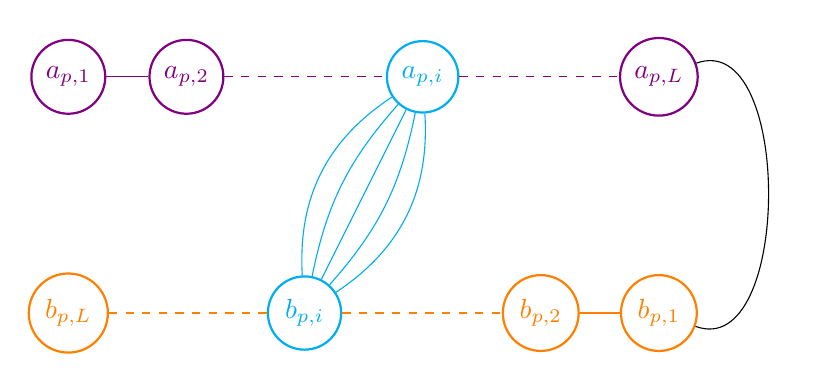
\begin{tikzpicture}[node distance={15mm}, main/.style = {draw, thick, circle}]
			\node[main, color=violet] (1) {$a_{p,1}$};
			\node[below of = 1] (phantom) {};
			\node[main, right of = 1, color=violet] (2) {$a_{p,2}$};
			\node[right of = 2] (3) {};
			\node[main, right of = 3, color=cyan] (4) {$a_{p,i}$};
			\node[right of = 4] (5) {};
			\node[main, right of = 5, color=violet] (6) {$a_{p,L}$};
			\node[main, below of = phantom, color=orange] (7) {$b_{p,L}$};
			\node[right of = 7] (8) {};
			\node[main, right of = 8, color=cyan] (9) {$b_{p,i}$};
			\node[right of = 9] (10) {};
			\node[main, right of = 10, color=orange] (11) {$b_{p,2}$};
			\node[main, right of = 11, color=orange] (12) {$b_{p,1}$};
			\draw[color=violet] (1) edge (2);
			\draw[color=orange] (12) edge (11);
			\draw[color=violet, dashed] (2) edge (4);
			\draw[color=violet, dashed] (4) edge (6);
			\draw[color=orange, dashed] (7) edge (9);
			\draw[color=orange, dashed] (9) edge (11);
			\draw[color=black, bend right = 110] (12) edge (6);
			\draw[color=cyan] (4) edge (9);
			\draw[color=cyan, bend right = 15] (4) edge (9);
			\draw[color=cyan, bend left = 15] (4) edge (9);
			\draw[color=cyan, bend right = 30] (4) edge (9);
			\draw[color=cyan, bend left = 30] (4) edge (9);
		\end{tikzpicture}
		\caption{Illustration of the shortening system for $S_{p,i}$.}
		\label{shortening}
	\end{figure}
	
	\begin{enumerate}
		\item An initial segment between $a_{p,1}$ and $a_{p,i}$ of $p$ plus the final segment between $b_{p,L}$ and $b_{p,i}$. Also we will scale these down by $(1 + \epsilon) L$.
		\item We use the flow for the commodity $(a_{p,i}, b_{p,i}, f_{p}) \in \mathcal{U}$ with flow of a size $\frac{f_{p}}{L(1 + \epsilon)}$.
	\end{enumerate}
	
	Now the sum of flow between $a_{p,i}$ and $b_{p,i}$ over all flow systems $S_{p,i}$ is equal to $L \frac{f_{p}}{(1+\epsilon)L} = \frac{f_{p}}{(1+\epsilon)}$. Also for every $p \in \mathcal{O} \setminus \mathcal{O}'$ we scale down the flow by $(1 + \epsilon)$.
	
	Think about the optimal feasible flow for $\mathcal{U}$. It has these properties:
	
	\begin{itemize}
		\item $\forall e \in E$ the flow in $e$ is $\leq 1$. (It is feasible solution.)
		\item $\forall (a, b, f) \in \mathcal{U}$ the flow between $a$ and $b$ is $\geq \frac{f}{2F}$. (Due to the claim for BMFP instance.)
	\end{itemize}
	
	Therefore by scaling these down by $\frac{\epsilon}{1 + \epsilon}$ we get the amount we need for all $S_{p,i}$'s. Simply if we rewrite $\frac{f_{p}}{L(1 + \epsilon)} = \frac{f_{p}}{2F(1 + \epsilon)}\epsilon$. Hence for an edge $e \in E$ the amount of flow on $e$ due to the "shortcuts" is $\leq \frac{\epsilon}{1+\epsilon}$. Thus $\forall e \in E$ the total flow is $\leq \frac{1}{1 + \epsilon} = \frac{\epsilon}{1+\epsilon} = 1$. Note that these are really shortcuts, because we have used the previous claim to obtain such solution for BMFP.
\end{proof}

\section{Bounded greedy algorithm}

Lets take a graph $G = (V,E)$ its flow number $F = F(G)$ and consider edge disjoint path problem on such $G$ with commodities $(s_{i}, t_{i})$ for $i \in [k]$. We will use the Greedy algorithm already mentioned, but with the parameter $4F$ instead.

Now we will analyze how the algorithm goes. Let $\mathcal{B}$ be the paths of Greedy($4F$) and $\mathcal{O}$ the paths in optimal solution. We may look at the optimal paths as an instance of a flow problem. Therefore we will use shortening lemma with $\epsilon = 1$ on the flow system $\mathcal{O}$. So let $\mathcal{O}'$ be the resulting flow system. We may see that both $\mathcal{O}'$ and $\mathcal{B}$ uses paths with lengths at most $4F$.

For $(s_{i}, t_{i}) \in \mathcal{O}' \setminus \mathcal{B}$ consider a path $p$ connecting $s_{i}$ and $t_{i}$. Because it was not used by the algorithm there must $\exists q \in \mathcal{B}$ such that $q \cap p \neq \emptyset$. We may say that \textit{"$q$ is a witness of $(s_{i},t_{i})$ of weight $f_{p}$"}.

\begin{observ}
	For every $(s_{i}, t_{i}) \in \mathcal{O}' \setminus \mathcal{B}$ there exists witnesses for $(s_{i}, t_{i})$ in $\mathcal{B}$ of total weight $\geq 1/2$.
\end{observ}

\begin{observ}
	Any path in $\mathcal{B}$ serves as a witness of weight $\leq 4F$.
\end{observ}

Therefore altogether we get the following:

$$
\begin{aligned}
	|\mathcal{O}| &\leq |\mathcal{O}' \setminus \mathcal{B}| + |\mathcal{B}| \\
	 &\leq 8F |\mathcal{B}| + |\mathcal{B}| \\
	 & = O(F) |\mathcal{B}|
\end{aligned}
$$

\begin{thm}
	The approximation ratio of the BGA($4F$) is $O(F)$.
\end{thm}

\section{NP hardness of the problem}


In this section we will take a look at the hardness of this problem. That is $\forall \epsilon > 0$ it is NP-hard to approximate DIR-EDP (directed edge disjoint problem) within $n^{1/2 - \epsilon}$. We may show this by the hardness of the 2-DIR-EDP. Firstly we construct a $l \times l$ mash as depicted on the picture \ref{l_by_l_mesh}. Now we will replace each vertex inside the mesh with a special graph $H$ that is shown on the picture \ref{h subgraph}.

\begin{figure}[!ht]
	\begin{subfigure}{0.6\textwidth}\centering
		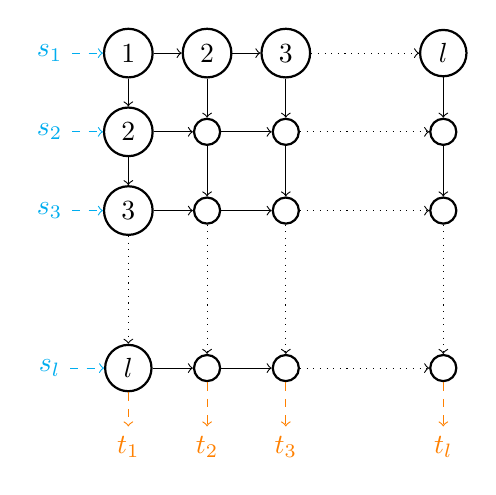
\begin{tikzpicture}[node distance={10mm}, main/.style = {draw, thick, circle}]
			\node[main] (11) {1};
			\node[main, right of = 11] (21) {2};
			\node[main, right of = 21] (31) {3};
			\node[right of = 31] (i1) {};
			\node[main, right of = i1] (l1) {$l$};
			
			\node[main, below of = 11] (12) {2};
			\node[main, right of = 12] (22) {};
			\node[main, right of = 22] (32) {};
			\node[right of = 32] (i2) {};
			\node[main, right of = i2] (l2) {};
			
			\node[main, below of = 12] (13) {3};
			\node[main, right of = 13] (23) {};
			\node[main, right of = 23] (33) {};
			\node[right of = 33] (i3) {};
			\node[main, right of = i3] (l3) {};
			
			\node[below of = 13] (1i) {};
			\node[right of = 1i] (2i) {};
			\node[right of = 2i] (3i) {};
			\node[right of = 3i] (ii) {};
			\node[right of = ii] (li) {};
			
			\node[main, below of = 1i] (1l) {$l$};
			\node[main, right of = 1l] (2l) {};
			\node[main, right of = 2l] (3l) {};
			\node[right of = 3l] (il) {};
			\node[main, right of = il] (ll) {};
		 	
			\draw[->] (11) edge (21);
			\draw[->] (21) edge (31);
			\draw[->, dotted] (31) edge (l1);
			
			\draw[->] (12) edge (22);
			\draw[->] (22) edge (32);
			\draw[->, dotted] (32) edge (l2);
			
			\draw[->] (13) edge (23);
			\draw[->] (23) edge (33);
			\draw[->, dotted] (33) edge (l3);
			
			\draw[->] (1l) edge (2l);
			\draw[->] (2l) edge (3l);
			\draw[->, dotted] (3l) edge (ll);
			
			\draw[->] (11) edge (12);
			\draw[->] (12) edge (13);
			\draw[->, dotted] (13) edge (1l);
			
			\draw[->] (21) edge (22);
			\draw[->] (22) edge (23);
			\draw[->, dotted] (23) edge (2l);
			
			\draw[->] (31) edge (32);
			\draw[->] (32) edge (33);
			\draw[->, dotted] (33) edge (3l);
			
			\draw[->] (l1) edge (l2);
			\draw[->] (l2) edge (l3);
			\draw[->, dotted] (l3) edge (ll);
			
			\node[left of = 11] (s1) {\textcolor{cyan}{$s_1$}};
			\node[left of = 12] (s2) {\textcolor{cyan}{$s_2$}};
			\node[left of = 13] (s3) {\textcolor{cyan}{$s_3$}};
			\node[left of = 1l] (sl) {\textcolor{cyan}{$s_l$}};
			\draw[->, color=cyan, dashed] (s1) edge (11);
			\draw[->, color=cyan, dashed] (s2) edge (12);
			\draw[->, color=cyan, dashed] (s3) edge (13);
			\draw[->, color=cyan, dashed] (sl) edge (1l);
			
			\node[below of = 1l] (t1) {\textcolor{orange}{$t_1$}};
			\node[below of = 2l] (t2) {\textcolor{orange}{$t_2$}};
			\node[below of = 3l] (t3) {\textcolor{orange}{$t_3$}};
			\node[below of = ll] (tl) {\textcolor{orange}{$t_l$}};
			\draw[->, color=orange, dashed] (1l) edge (t1);
			\draw[->, color=orange, dashed] (2l) edge (t2);
			\draw[->, color=orange, dashed] (3l) edge (t3);
			\draw[->, color=orange, dashed] (ll) edge (tl);
		\end{tikzpicture}
		\caption{$l \times l$ original mesh.}
		\label{l_by_l_mesh}
	\end{subfigure}
	\begin{subfigure}{0.3\textwidth}\centering
		\begin{tikzpicture}[node distance={10mm}, main/.style = {draw, thick, circle}]
			\node (h) {$H$};
			\node[main, left of = h] (2) {};
			\node[main, above of = h] (3) {};
			\node[main, right of = h] (4) {};
			\node[main, below of = h] (5) {};
			\node[left of = 2] (1) {};
			\node[above of = 3] (6) {};
			\node[right of = 4] (7) {};
			\node[below of = 5] (8) {};
			
			\draw[->] (1) edge (2);
			\draw[->] (6) edge (3);
			\draw[->] (4) edge (7);
			\draw[->] (5) edge (8);
			\draw[bend left = 40] (2) edge (3);
			\draw[bend left = 40] (3) edge (4);
			\draw[bend left = 40] (4) edge (5);
			\draw[bend left = 40] (5) edge (2);
		\end{tikzpicture}
		\caption{Replacement graph $H$.}
		\label{h subgraph}
	\end{subfigure}
	\caption{Separate parts to create graph $G$.}
\end{figure}

With this construction the graph $G$ contains $|V(G)| = l \times l \times k$ and let $k = |V(H)|$ then set $n = k^{1/2 \epsilon}$ and $l = n$. With this $|V(G)|$ is asymptotically $n$ (we were not counting sources and targets).

\begin{observ}
	If this 2-DIR-EDP of instance $H$ is YES-instance, then we can connect all $l$ pairs $s_i t_i$. by edge disjoint paths.	
\end{observ}

\begin{observ}
	If this 2-DIR-EDP of instance $H$ is NO-instance, then we can connect at most 1 $s_i t_i$ pair.
\end{observ}

With all these observation we see that from 2-DIR-EDP $\Rightarrow n^{1/2 - \epsilon}$ approximation.

\subsection{2-DIR-EDP is NP-hard}

As we have shown te NP-hardness of general DIR-EDP to 2-DIR-EDP we will now show the reduction from 3-SAT to 2-DIR-EDP. That is we have a formula $F$ in CNF (conjecttion of clauses which are disjunction of 3 literals).

We have $k$ variables $x_1, x_2, \dots, x_k$ and $l$ clauses $t_1, t_2, \dots, t_l$. And we will show how the graph will be constructed. Firstly for every variable we will construct a gadget that has one entering and one leaving vertex and two separate paths, where on these paths are represented negative and positive occurrences of this variable. This can be seen on the picture \ref{variable gadget}. These gadgets will be connected sequentially by exactly one edge.

\begin{figure}[!ht]\centering
	\begin{subfigure}{0.3\textwidth}\centering
		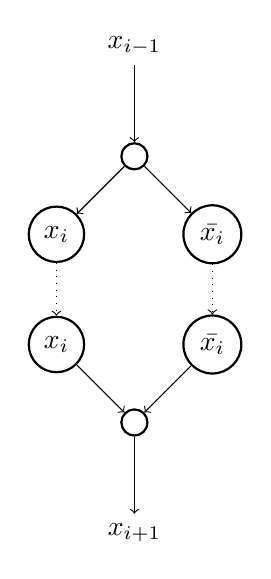
\begin{tikzpicture}[node distance={14mm}, main/.style = {draw, thick, circle}]
			\node (x-1) {$x_{i - 1}$};
			\node[main, below of = x-1] (e) {};
			\node[main, below left of = e] (x) {$x_i$};
			\node[main, below right of = e] (notx) {$\bar{x_i}$};
			\node[main, below of = x] (phx) {$x_i$};
			\node[main, below of = notx] (phnotx) {$\bar{x_i}$};
			\node[main, below right of = phx] (end) {};
			\node[below of = end] (x+1) {$x_{i + 1}$};
			\draw[->] (x-1) edge (e);
			\draw[->] (end) edge (x+1);
			\draw[->] (e) edge (x);
			\draw[->] (e) edge (notx);
			\draw[->, dotted] (x) edge (phx);
			\draw[->, dotted] (notx) edge (phnotx);
			\draw[->] (phx) edge (end);
			\draw[->] (phnotx) edge (end);
		\end{tikzpicture}
		\caption{Gadget for variables $x_i$.}
		\label{variable gadget}
	\end{subfigure}
	\begin{subfigure}{0.68\textwidth}\centering
		\begin{tikzpicture}[node distance={13mm}, main/.style = {draw, thick, circle}]
			\node[main] (startx0) {};
			\node[below of = startx0] (labelx0) {$x_0$};
			\node[main, below left of = startx0] (x0) {};
			\node[main, below right of = startx0] (notx0) {};
			\node[main, below of = x0] (phx0) {};
			\node[main, below of = notx0] (phnotx0) {};
			\node[main, below right of = phx0] (endx0) {};
			
			\node[below of = endx0] (gap) {};
			
			\node[main, below of = gap] (startxk) {};
			\node[below of = startxk] (labelxk) {$x_k$};
			\node[main, below left of = startxk] (xk) {};
			\node[main, below right of = startxk] (notxk) {};
			\node[main, below of = xk] (phxk) {};
			\node[main, below of = notxk] (phnotxk) {};
			\node[main, below right of = phxk] (endxk) {};
			
			\node[left of = endxk] (phantom0) {};
			\node[left of = phantom0] (phantom1) {};
			\node[left of = phantom1] (phantom2) {};
			\node[main, left of = phantom2] (c0) {$c_0$};
			\node[main, above of = c0] (c1) {$c_1$};
			\node[main, above of = c1] (c2) {$c_2$};
			\node[above of = c2] (gapc) {};
			\node[main, above of = gapc] (cl) {$c_l$};
			
			\draw[->] (startx0) edge (x0);
			\draw[->] (startx0) edge (notx0);
			\draw[->] (x0) edge (phx0);
			\draw[->] (notx0) edge (phnotx0);
			\draw[->] (phx0) edge (endx0);
			\draw[->] (phnotx0) edge (endx0);
			
			\draw[->, dotted] (endx0) edge (startxk);
			
			\draw[->] (startxk) edge (xk);
			\draw[->] (startxk) edge (notxk);
			\draw[->] (xk) edge (phxk);
			\draw[->] (notxk) edge (phnotxk);
			\draw[->] (phxk) edge (endxk);
			\draw[->] (phnotxk) edge (endxk);
			
			\draw[->, bend left = 60] (endxk) edge (c0);
			\draw[->] (c0) edge (c1);
			\draw[->, bend right = 50] (c0) edge (c1);
			\draw[->, bend left = 50] (c0) edge (c1);
			\draw[->] (c1) edge (c2);
			\draw[->, bend right = 50] (c1) edge (c2);
			\draw[->, bend left = 50] (c1) edge (c2);
			\draw[->, dotted] (c2) edge (cl);
		\end{tikzpicture}
		\caption{Scheme of variables and clauses.}
		\label{clause var scheme}
	\end{subfigure}
	\caption{Gadgets for variables and for clauses.}
\end{figure}

And then for every clause we will have one vertex and every two consequent clauses will be connected by 3 edges. These will represent the given literals. Also the last variable will be connected to the first clause. The scheme can be seen on the picture \ref{clause var scheme}. Now we only need to connect these gadgets together.

For that we will introduce \textbf{switch} gadget which connects the two previously mentioned gadgets. The exact construction of the switch is shown on the picture \ref{switch}. But it is enough to see the scheme of the switch on the picture \ref{scheme analyse}.

\begin{figure}[!ht]\centering
	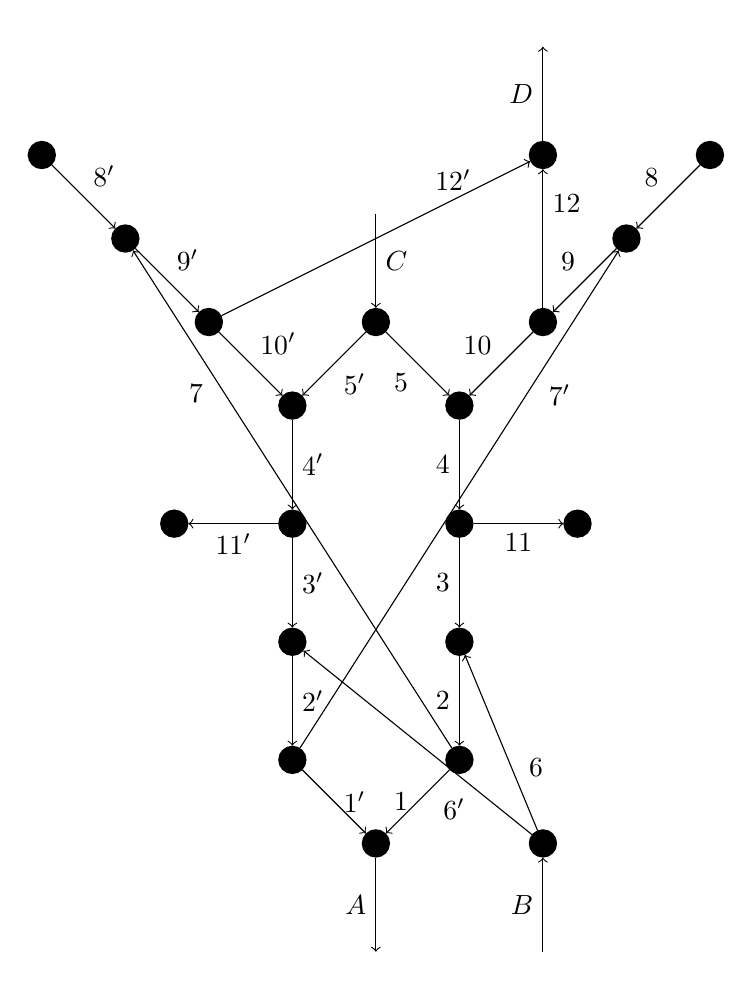
\begin{tikzpicture}[node distance={15mm}, main/.style = {draw, thick, circle, fill}]
		%% NODES
		% Start
		\node (1) {}; % Invisible start.
		\node[main, below of = 1] (2) {};
		% Left path
		\node[main, below left of = 2] (3) {};
		\node[main, below of = 3] (4) {};
		\node[main, below of = 4] (5) {};
		\node[main, below of = 5] (6) {};
		% Right path
		\node[main, below right of = 2] (3') {};
		\node[main, below of = 3'] (4') {};
		\node[main, below of = 4'] (5') {};
		\node[main, below of = 5'] (6') {};
		% End
		\node[main, below right of = 6] (7) {};
		\node[below of = 7] (8) {}; % Invisible end
		% Left wing		
		\node[main, above left of = 3] (9) {};
		\node[main, above left of = 9] (10) {};
		\node[main, above left of = 10] (11) {};
		% Right wing
		\node[main, above right of = 3'] (9') {};
		\node[main, above right of = 9'] (10') {};
		\node[main, above right of = 10'] (11') {};
		% Left arm
		\node[main, left of = 4] (12) {};
		% Right arm
		\node[main, right of = 4'] (12') {};
		% Rest of the graph.
		\node[main, above left of = 10'] (upper) {};
		\node[above of = upper] (ph-upper) {}; % Invisible upper
		\node[main, below right of = 6'] (lower) {};
		\node[below of = lower] (ph-lower) {}; % Invisible lower
		%% --S
		% Main two paths.
		\draw[->] (1) -- (2) node[midway, right] {$C$};
		\draw[->] (7) -- (8) node[midway, left] {$A$};
		\draw[->] (2) -- (3) node[midway, below right] {$5'$};
		\draw[->] (3) -- (4) node[midway, right] {$4'$};
		\draw[->] (4) -- (5) node[midway, right] {$3'$};
		\draw[->] (5) -- (6) node[midway, right] {$2'$};
		\draw[->] (6) -- (7) node[midway, right] {$1'$};
		\draw[->] (2) -- (3') node[midway, below left] {$5$};
		\draw[->] (3') -- (4') node[midway, left] {$4$};
		\draw[->] (4') -- (5') node[midway, left] {$3$};
		\draw[->] (5') -- (6') node[midway, left] {$2$};
		\draw[->] (6') -- (7) node[midway, left] {$1$};
		% Wings.
		\draw[->] (11) -- (10) node[midway, above right] {$8'$};
		\draw[->] (10) -- (9) node[midway, above right] {$9'$};
		\draw[->] (9) -- (3) node[midway, above right] {$10'$};
		\draw[->] (11') -- (10') node[midway, above left] {$8$};
		\draw[->] (10') -- (9') node[midway, above left] {$9$};
		\draw[->] (9') -- (3') node[midway, above left] {$10$};
		% Arms
		\draw[->] (4) -- (12) node[midway, below] {$11'$};
		\draw[->] (4') -- (12') node[midway, below] {$11$};
		% Rest of the graph.
		\draw[->] (ph-lower) -- (lower) node[midway, left] {$B$};
		\draw[->] (lower) -- (5) node[near start, below left]{$6'$};
		\draw[->] (lower) -- (5') node[near start, above right] {$6$};
		\draw[->] (upper) -- (ph-upper) node[midway, left] {$D$};
		\draw[->] (9) -- (upper) node[near end, above] {$12'$};
		\draw[->] (9') -- (upper) node[near end, right] {$12$};
		% The remaining two --s.
		\draw[->] (6) -- (10') node[near end, below right] {$7'$};
		\draw[->] (6') -- (10) node[near end, below left] {$7$};
	\end{tikzpicture}
	\caption{Switch construction.}
	\label{switch}
\end{figure}

\begin{figure}[!ht]\centering
	\begin{subfigure}{0.45\textwidth}\centering
		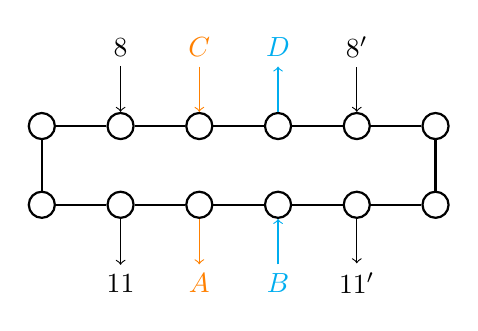
\begin{tikzpicture}[node distance={10mm}, main/.style = {draw, thick, circle}]
			\node[main] (O1) {};
			\node[main, right of = O1] (O2) {};
			\node[main, right of = O2] (O3) {};
			\node[main, right of = O3] (O4) {};
			\node[main, right of = O4] (O5) {};
			\node[main, right of = O5] (O6) {};
			\node[main, below of = O1] (O7) {};
			\node[main, right of = O7] (O8) {};
			\node[main, right of = O8] (O9) {};
			\node[main, right of = O9] (O10) {};
			\node[main, right of = O10] (O11) {};
			\node[main, right of = O11] (O12) {};
			
			\node[above of = O2] (8) {$8$};
			\node[above of = O3, color = orange] (C) {$C$};
			\node[above of = O4, color = cyan] (D) {$D$};
			\node[above of = O5] (8') {$8'$};
			\node[below of = O8] (11) {$11$};
			\node[below of = O9, color = orange] (A) {$A$};
			\node[below of = O10, color = cyan] (B) {$B$};
			\node[below of = O11] (11') {$11'$};
			
			\path[thick] (O1) edge (O2)
				(O2) edge (O3)
				(O3) edge (O4)
				(O4) edge (O5)
				(O5) edge (O6)
				(O7) edge (O8)
				(O7) edge (O1)
				(O8) edge (O9)
				(O9) edge (O10)
				(O10) edge (O11)
				(O11) edge (O12)
				(O12) edge (O6);
			\draw[->] (8) edge (O2);
			\draw[->, color = orange] (C) edge (O3);
			\draw[->, color = cyan] (O4) edge (D);
			\draw[->] (8') edge (O5);
			\draw[->] (O8) edge (11);
			\draw[->, color = orange] (O9) edge (A);
			\draw[->, color = cyan] (B) edge (O10);
			\draw[->] (O11) edge (11');
		\end{tikzpicture}
		\caption{Scheme for analyzing.}
		\label{scheme analyse}
	\end{subfigure}
	\begin{subfigure}{0.45\textwidth}\centering
		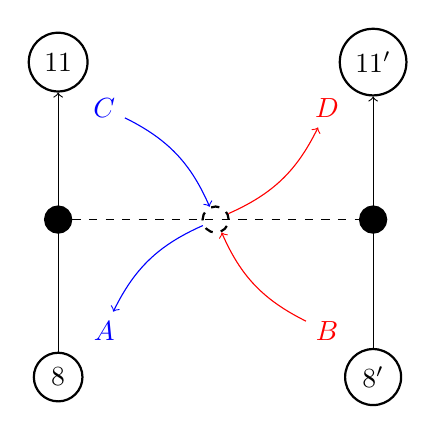
\begin{tikzpicture}[node distance={20mm}, main/.style = {draw, thick, circle}]
			\node[main] (8) {$8$};
			\node[main, fill, above of = 8] (phantom) {};
			\node[main, above of = phantom] (11) {$11$};
			\node[main, dashed, right of = phantom] (mid) {};
			\node[main, fill, right of = mid] (phantom') {};
			\node[main, below of = phantom'] (8') {$8'$};
			\node[main, above of = phantom'] (11') {$11'$};
			\node[above right of = mid, color = red] (D) {$D$};
			\node[above left of = mid, color = blue] (C) {$C$};
			\node[below right of = mid, color = red] (B) {$B$};
			\node[below left of = mid, color = blue] (A) {$A$};
			
			\draw[->] (8) edge (11);
			\draw[->] (8') edge (11');
			\draw[dashed] (phantom) edge (phantom');
			\draw[->, bend right = 20, color = blue] (mid) edge (A);
			\draw[->, bend left = 20, color = red] (B) edge (mid);
			\draw[->, bend left = 20, color = blue] (C) edge (mid);
			\draw[->, bend right = 20, color = red] (mid) edge (D);
		\end{tikzpicture}
		\caption{Drawn switch scheme.}
	\end{subfigure}
	\caption{Switch scheme.}
	\label{switch scheme}
\end{figure}


We may see that the switch is a small graph with 4 "inputs" $B, C, 8, 8'$ and 4 "outputs" $A, D, 11, 11'$. It can be shown that this graph has two following properties.

\begin{enumerate}
	\item If there are 2 edge disjoint paths one leaving at \textcolor{orange}{$A$} and the other entering at \textcolor{cyan}{$B$}, then the former is entering at \textcolor{orange}{$C$} and the later leaving at \textcolor{cyan}{$D$}. Look at the picture \ref{scheme analyse}.
	\item And exactly one more edge-disjoint path through the graph exists and it is either $8 \to 11$ or $8' \to 11'$.
\end{enumerate}

These switches can be connected by combining $A$ and $C$ and also $B$ and $D$. Therefore we insert the switches so $8 \to 11$ is for the variable in the clause gadget and the other ($8' \to 11'$) is replaced for the variable in the variable clause. After that we arbitrarily connect all switches together. Lastly we also insert vertices \textcolor{violet}{$W, X, Y, Z$} as shown on the global picture \ref{global scheme}.

\begin{figure}[!ht]\centering
		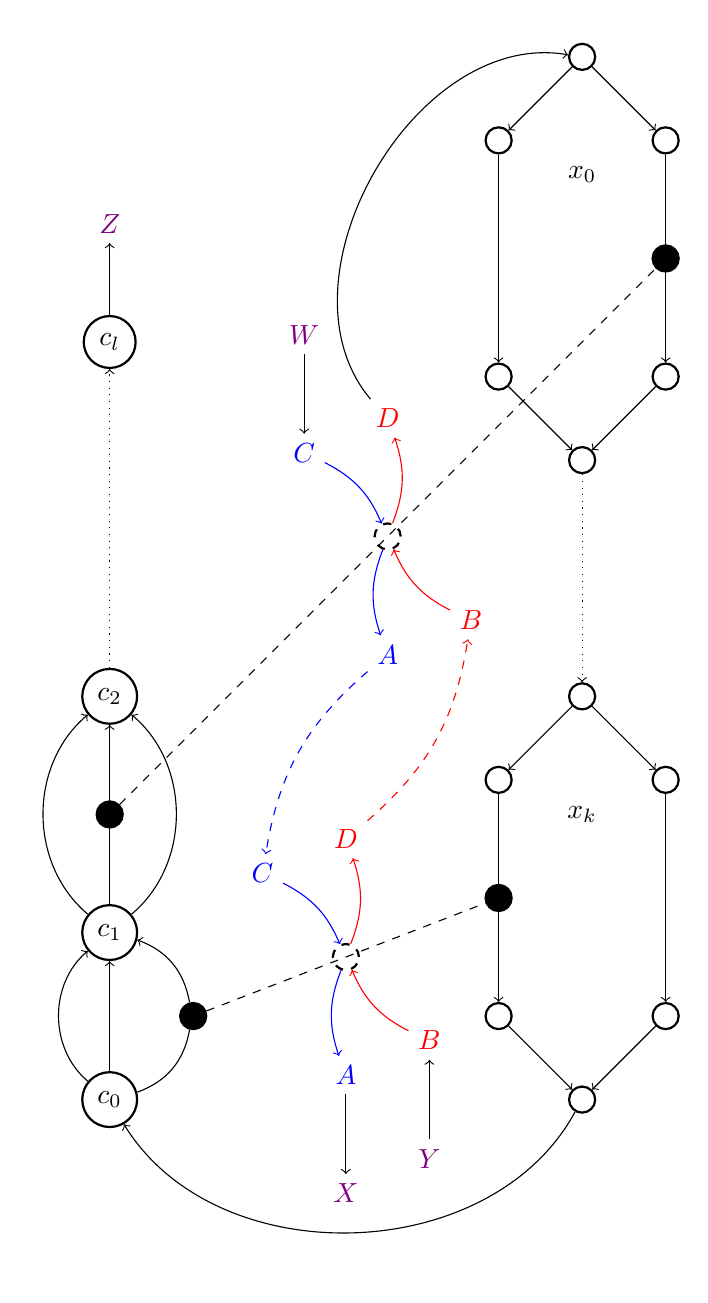
\begin{tikzpicture}[node distance={15mm}, main/.style = {draw, thick, circle}]
		\node[main] (startx0) {};
		\node[below of = startx0] (labelx0) {$x_0$};
		\node[main, below left of = startx0] (x0) {};
		\node[main, below right of = startx0] (notx0) {};
		\node[main, fill, below of = notx0] (dotx0) {};
		\node[below of = x0] (invdotx0) {};
		\node[main, below of = dotx0] (phnotx0) {};
		\node[main, below of = invdotx0] (phx0) {};
		\node[main, below right of = phx0] (endx0) {};
		
		\node[below of = endx0] (gap) {};
		
		\node[main, below of = gap] (startxk) {};
		\node[below of = startxk] (labelxk) {$x_k$};
		\node[main, below left of = startxk] (xk) {};
		\node[main, below right of = startxk] (notxk) {};
		\node[main, fill, below of = xk] (dotxk) {};
		\node[below of = notxk] (invdotxk) {};
		\node[main, below of = dotxk] (phxk) {};
		\node[main, below of = invdotxk] (phnotxk) {};
		\node[main, below right of = phxk] (endxk) {};
		
		\node[left of = endxk] (phantom0) {};
		\node[left of = phantom0] (phantom1) {};
		\node[left of = phantom1] (phantom2) {};
		\node[main, left of = phantom2] (c0) {$c_0$};
		\node[main, fill, above right of = c0] (dotc0) {};
		\node[main, above left of = dotc0] (c1) {$c_1$};
		\node[main, fill, above of = c1] (dotc1) {};
		\node[main, above of = dotc1] (c2) {$c_2$};
		\node[above of = c2] (gapc) {};
		\node[above of = gapc] (gapcc) {};
		\node[main, above of = gapcc] (cl) {$c_l$};
		
		\draw[->] (startx0) edge (x0);
		\draw[->] (startx0) edge (notx0);
		\draw[->] (x0) edge (phx0);
		\draw[->] (notx0) edge (phnotx0);
		\draw[->] (phx0) edge (endx0);
		\draw[->] (phnotx0) edge (endx0);
		
		\draw[->, dotted] (endx0) edge (startxk);
		
		\draw[->] (startxk) edge (xk);
		\draw[->] (startxk) edge (notxk);
		\draw[->] (xk) edge (phxk);
		\draw[->] (notxk) edge (phnotxk);
		\draw[->] (phxk) edge (endxk);
		\draw[->] (phnotxk) edge (endxk);
		
		\draw[->, bend left = 60] (endxk) edge (c0);
		\draw[->] (c0) edge (c1);
		\draw[bend right = 30] (c0) edge (dotc0);
		\draw[->, bend right = 30] (dotc0) edge (c1);
		\draw[->, bend left = 50] (c0) edge (c1);
		\draw[->] (c1) edge (c2);
		\draw[->, bend right = 50] (c1) edge (c2);
		\draw[->, bend left = 50] (c1) edge (c2);
		\draw[->, dotted] (c2) edge (cl);
		
		\draw[dashed] (dotc0) -- (dotxk) node[main, midway] (mid0) {};
		\draw[dashed] (dotc1) -- (dotx0) node[main, midway] (mid1) {};
		
		\node[above left of = mid0, color = blue] (C0) {$C$};
		\node[above of = mid0, color = red] (D0) {$D$};
		\node[below right of = mid0, color = red] (B0) {$B$};
		\node[below of = mid0, color = blue] (A0) {$A$};
		
		\node[above left of = mid1, color = blue] (C1) {$C$};
		\node[above of = mid1, color = red] (D1) {$D$};
		\node[below right of = mid1, color = red] (B1) {$B$};
		\node[below of = mid1, color = blue] (A1) {$A$};
		
		\draw[->, bend left = 20, color = blue] (C0) edge (mid0);
		\draw[->, bend left = 20, color = red] (B0) edge (mid0);
		\draw[->, bend right = 20, color = blue] (mid0) edge (A0);
		\draw[->, bend right = 20, color = red] (mid0) edge (D0);
		
		\draw[->, bend left = 20, color = blue] (C1) edge (mid1);
		\draw[->, bend left = 20, color = red] (B1) edge (mid1);
		\draw[->, bend right = 20, color = blue] (mid1) edge (A1);
		\draw[->, bend right = 20, color = red] (mid1) edge (D1);
		
		\draw[->, dashed, bend right = 20, color = red] (D0) edge (B1);
		\draw[->, dashed, bend right = 20, color = blue] (A1) edge (C0);
		
		\node[below of = A0, color = violet] (X) {$X$};
		\node[below of = B0, color = violet] (Y) {$Y$};
		\node[above of = cl, color = violet] (Z) {$Z$};
		\node[above of = C1, color = violet] (W) {$W$};
		
		\draw[->] (A0) edge (X);
		\draw[->] (Y) edge (B0);
		\draw[->] (W) edge (C1);
		\draw[->] (cl) edge (Z);
		\draw[->, bend left = 70] (D1) edge (startx0);
	\end{tikzpicture}
	\caption{Global scheme of the 3-SAT.}
	\label{global scheme}
\end{figure}

\begin{claim}
	$F$ is satisfiable $\Leftrightarrow$ there are edge disjoint paths from $W$ to $X$ and from $Y$ to $Z$.
\end{claim}

That can be seen on the global scheme. Important note is that for example if $x_i$ is set to true then the variable gadget uses $\bar{x_i}$ in the subgraph of $G$. Generally it uses the other path so it enforces the correct values in the clauses and also the other way around.

	\chapter{$L$-bounded cuts}

In this chapter we will consider a new problem which is length bounded cuts. This problem is NP-hard.

\begin{itemize}[]
	\item \textbf{INPUT} $G = (V,E)$, $s,t \in V$, $L \in \N$.
	\item \textbf{OUTPUT} $F \subseteq E$ such that $d_{G \setminus F}(s,t) > L$.
	\item \textbf{OBJECTIVE} $\min (|F|)$.
\end{itemize}

Lets see an easy example of a graph $G$ as shown on the picture \ref{l-bounded cut} and for $L = 4$. There can actually be two minimal $L$-bounded cuts. The \textcolor{orange}{first} one is actually not a "real" cut, but the \textcolor{cyan}{second} one is.

\begin{figure}[!ht]\centering
	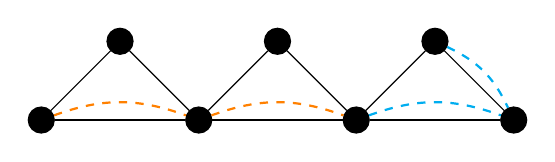
\begin{tikzpicture}[node distance={10mm}, main/.style = {draw, fill, circle}]
		\node[main] (1) {};
		\node[right of = 1] (1a) {};
		\node[main, above of = 1a] (1b) {};
		\node[main, right of = 1a] (2) {};
		\node[right of = 2] (2a) {};
		\node[main, above of = 2a] (2b) {};
		\node[main, right of = 2a] (3) {};
		\node[right of = 3] (3a) {};
		\node[main, above of = 3a] (3b) {};
		\node[main, right of = 3a] (4) {};
		
		\draw (1) edge (2);
		\draw (1) edge (1b);
		\draw (1b) edge (2);
		
		\draw (2) edge (3);
		\draw (2) edge (2b);
		\draw (2b) edge (3);
		
		\draw (3) edge (4);
		\draw (3) edge (3b);
		\draw (3b) edge (4);
		
		\draw[color = orange, thick, bend left = 20, dashed] (1) edge (2);
		\draw[color = orange, thick, bend left = 20, dashed] (2) edge (3);
		
		\draw[color = cyan, thick, bend left = 20, dashed] (3) edge (4);
		\draw[color = cyan, thick, bend left = 20, dashed] (3b) edge (4);
	\end{tikzpicture}
	\caption{Example of $L$-bounded cut. The cut is drawn by a multiple dashed edge.}
	\label{l-bounded cut}
\end{figure}


\section{$L$-bounded flow}

For $L$-bounded cut there is also the opposite problem which is in P and it is the $L$-bounded flow.

\begin{itemize}[]
	\item \textbf{INPUT} $G = (V,E)$, $s,t \in V$, $L \in \N$.
	\item \textbf{OUTPUT} Flow between $s-t$ that can be decomposed into paths of length $\leq L$.
	\item \textbf{OBJECTIVE} $\max$ the flow.
\end{itemize}

We will also show us an example for a graph $G$ depicted on the picture \ref{l-bounded flow} for $L = 3k$. We may see that $L$-cut is $k+1$ since we may delete \textcolor{cyan}{these edges} but also \textcolor{orange}{the bottom ones}. On the other hand $L$-flow is at most 2.

\begin{figure}[!ht]\centering
	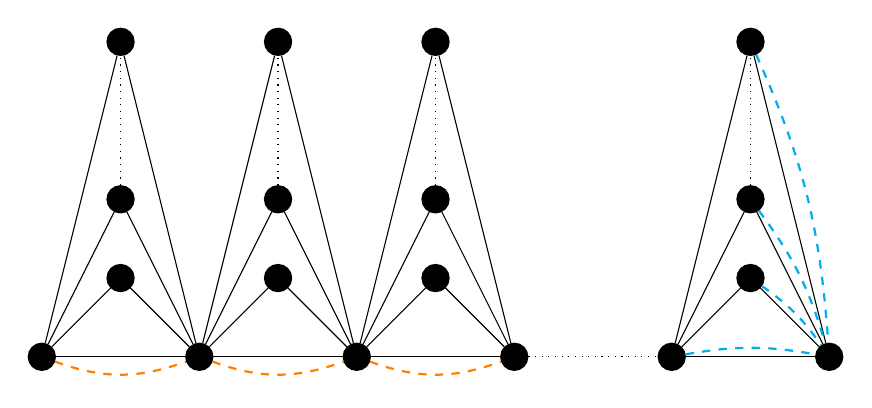
\begin{tikzpicture}[node distance={10mm}, main/.style = {draw, thick, fill, circle}]
		\node[main] (1) {};
		\node[right of = 1] (1a) {};
		\node[main, above of = 1a] (1b) {};
		
		\node[main, above of = 1b] (1c) {};
		\node[above of = 1c] (1d) {};
		\node[main, above of = 1d] (1e) {};
		
		\node[main, right of = 1a] (2) {};
		\node[right of = 2] (2a) {};
		\node[main, above of = 2a] (2b) {};
		
		\node[main, above of = 2b] (2c) {};
		\node[above of = 2c] (2d) {};
		\node[main, above of = 2d] (2e) {};
		
		\node[main, right of = 2a] (3) {};
		\node[right of = 3] (3a) {};
		\node[main, above of = 3a] (3b) {};
		
		\node[main, above of = 3b] (3c) {};
		\node[above of = 3c] (3d) {};
		\node[main, above of = 3d] (3e) {};
		
		\node[main, right of = 3a] (4) {};
		
		\node[right of = 4] (phantom) {};
		
		\node[main, right of = phantom] (k) {};
		\node[right of = k] (ka) {};
		\node[main, above of = ka] (kb) {};
		
		\node[main, above of = kb] (kc) {};
		\node[above of = kc] (kd) {};
		\node[main, above of = kd] (ke) {};
		
		\node[main, right of = ka] (k+1) {};
		
		\draw (1) edge (2);
		\draw (1) edge (1b);
		\draw (1b) edge (2);
		\draw (1) edge (1c);
		\draw (1c) edge (2);
		\draw (1) edge (1e);
		\draw (1e) edge (2);
		\draw[dotted] (1c) edge (1e);
		
		\draw (2) edge (3);
		\draw (2) edge (2b);
		\draw (2b) edge (3);
		\draw (2) edge (2c);
		\draw (2c) edge (3);
		\draw (2) edge (2e);
		\draw (2e) edge (3);
		\draw[dotted] (2c) edge (2e);
		
		\draw (3) edge (4);
		\draw (3) edge (3b);
		\draw (3b) edge (4);
		\draw (3) edge (3c);
		\draw (3c) edge (4);
		\draw (3) edge (3e);
		\draw (3e) edge (4);
		\draw[dotted] (3c) edge (3e);
		
		\draw[dotted] (4) edge (k);
		
		\draw (k) edge (k+1);
		\draw (k) edge (kb);
		\draw (kb) edge (k+1);
		\draw (k) edge (kc);
		\draw (kc) edge (k+1);
		\draw (k) edge (ke);
		\draw (ke) edge (k+1);
		\draw[dotted] (kc) edge (ke);
		
		\draw[dashed, thick, color = cyan, bend left = 10] (k) edge (k+1);
		\draw[dashed, thick, color = cyan, bend left = 10] (kb) edge (k+1);
		\draw[dashed, thick, color = cyan, bend left = 10] (kc) edge (k+1);
		\draw[dashed, thick, color = cyan, bend left = 10] (ke) edge (k+1);
		
		\draw[dashed, thick, color = orange, bend right = 20] (1) edge (2);
		\draw[dashed, thick, color = orange, bend right = 20] (2) edge (3);
		\draw[dashed, thick, color = orange, bend right = 20] (3) edge (4);
	\end{tikzpicture}
	\caption{Example of $L$-bounded flow. Where there is $2k$ bottom vertices and $k$ upwards in each triangle. Cuts are represented by multi edges that are dashed.}
	\label{l-bounded flow}
\end{figure}

\begin{observ}
	Every $L$-bounded $s-t$ path uses at least $k$-edges from the bottom so max $L$-flow is at most 2.
\end{observ}

Therefore the difference between $L$-cut and $L$-flow can be at least $\sqrt{n}$.

\section{Approximation for $L$-cut}

Consider the following LP relaxation (denoted as (\textbf{D})). Alternatively the ILP will surely solve the problem. Lets denote $\mathcal{P}_L$ as the set of all $L$-bounded $s-t$ paths.

$$
\begin{aligned}
	\min \sum_{e \in E} x_e & \\
	\sum_{x \in p} x_e \geq 1 & \quad \forall p \in \mathcal{P}_L \\
	x_e \geq 0 & \quad \forall e \in E
\end{aligned}
$$

Also we can see what is the is the dual to this LP. Which will indeed solve $L$-flows. And we will denote it as (\textbf{P}).

$$
\begin{aligned}
	\max \sum_{p \in \mathcal{P}_L} f_p &\\
	\sum_{p: e \in p \in \mathcal{P}_L} f_p \leq 1 & \quad \forall e \in E\\
	f_p \geq 0 & \quad \forall p \in \mathcal{P}_L
\end{aligned}
$$

We may ask ourselves what is the integrality gap? From the instance shown on the picture \ref{l-bounded flow} we already saw that the max $L$-flow is $2$ and min $L$-cut is about $c \sqrt{n}$. Because of the duality we know the $L$-flow is the same as fractional $L$-cut, therefore the integrality gap is $\geq \Omega (\sqrt{n})$.

\subsection{$L$-approximations}

We can create multiple quite simple algorithms for solving such problem. These all will be approximation algorithms.

\begin{algorithm}
	\caption{ \texttt{(1)} $L$-bounded cut approximation}
	\begin{algorithmic}[1]
		\Require $G = (V,E)$
		\Ensure $L$-bounded cut.
		\While{$\exists L$-bounded $s-t$ path $p$ in $G$}
			\State Remove all edges of $p$.
		\EndWhile
	\end{algorithmic}
\end{algorithm}

\begin{observ}
	While the OPT $\geq k$ therefore it is $L$-approximation. Since the $k$ is the number of $L$-paths.
\end{observ}

\begin{algorithm}
	\caption{ \texttt{(2)} $L$-bounded cut approximation}
	\begin{algorithmic}[1]
		\Require $G = (V,E)$
		\Ensure $L$-bounded cut.
		\While{$d_g(s,t) \leq L$}
			\State $F := $ min cut in a subgraph of shortest paths.
			\State $G = G \setminus F$
		\EndWhile
	\end{algorithmic}
\end{algorithm}

We may clearly see that $|F| \leq \text{opt } L-\text{cut}$. Because we always need to delete some of these edges. We also always increase the shortest path by 1. Therefore it is an $L$-approximation since it is at max $L$ steps in the algorithm and for each it is at most the optimum.

\begin{algorithm}
	\caption{ \texttt{(3)} $L$-bounded cut approximation}
	\begin{algorithmic}[1]
		\Require $G = (V,E)$
		\Ensure $L$-bounded cut.
		\State Solve (\textbf{P}).
		\State $F := \{e \in E: \sum_{p : e \in p} f_p = 1\}$
	\end{algorithmic}
\end{algorithm}

In other words all saturated edges will form the $L$-cut. Now if $F$ wouldn't be an $L$-cut then the maximal flow was not maximal, since there is an $L$-path with non-saturated edge. Also $|F| \leq L (\max L-\text{flow})$ that is because every unit of a flow can saturate at most $L$ edges. And due to the duality $|F| \leq L (\max L-\text{flow}) \leq L (\min L-\text{cut})$. So once more we have obtained $L$-approximation.

\begin{algorithm}
	\caption{ \texttt{(4)} $L$-bounded cut approximation}
	\begin{algorithmic}[1]
		\Require $G = (V,E)$
		\Ensure $L$-bounded cut.
		\State Solve (\textbf{D}).
		\State $F := \left\{e \in E: x_e \geq \frac{1}{L}\right\}$
	\end{algorithmic}
\end{algorithm}

Due to the pigeonhole principle at least one edge in $L$-path has to have $\frac{1}{L}$, therefore it is a feasible solution. Because we are scaling the solution by the $L$ fraction we may see that $|F| \leq L (\min \text{ fractional } L-\text{cut}) \leq L \cdot \text{OPT}$. So we have another $L$-approximation.

There is an somewhat easy $L/2$-approximation only by combining \texttt{(1)} and \texttt{(2)}. This start with \texttt{(1)} with the bond lowered to $L/2$, then we switch to \texttt{(2)}.

\subsection{$n^{2/3}$-approximations}

Now what if we want to get approximation based on $n = |V(G)|$ instead of $L$. Can we create a $(n^{2/3})$-approximation. Firstly if $L \leq n^{2/3}$ then we are done by running $L$-approximation.

Otherwise we denote $\text{OPT}_L$ as the size of the optimal min $L$-cut. We may observe that for $L' < L$ it holds that $\text{OPT}_{L'} \leq \text{OPT}_L$ because all $L'$-paths are also $L$-paths.

The algorithm would be as follows. Firstly run $(n^{2/3})$-approximation from one of the four algorithms for this parameter. This will cost $O(n^{2/3} \cdot \text{OPT}_L)$.

Then by the theorem \ref{max flow bounded} we get that $l = n^{2/3}$ so the max flow is $\leq O(n^{2/3})$. Thus we can run the basic min cut problem on the whole graph which will also cost $O(n^{2/3} \cdot \text{OPT}_L)$ and also all together will be the same cost asymptotically.

\section{Integrality gap}

We will now create an instance for $L$-cut that has an integrality gap $n^{2/3}$. The scheme of the instance is depicted on picture \ref{huge integrality gap}. Firstly from $s$ node there are $n^{2/3}$ neighbors in the second layer. Next from the \textcolor{violet}{consecutive $n^{1/3}$ nodes} in the second layer have one common neighbor in the third layer. Therefore there is $n^{1/3}$ nodes in the third layer. After that it repeats for $n^{2/3}$ next layers and these middle parts form a \textcolor{cyan}{complete bipartite graph}. Then the last layer before $t$ is the same as from $s$, so it is a mirror image.

This is the underline structure where we add a \textcolor{orange}{shortcut} that skips every second layer. And lets say that there is $2k$ of the shortcuts.

\begin{figure}[!ht]\centering
	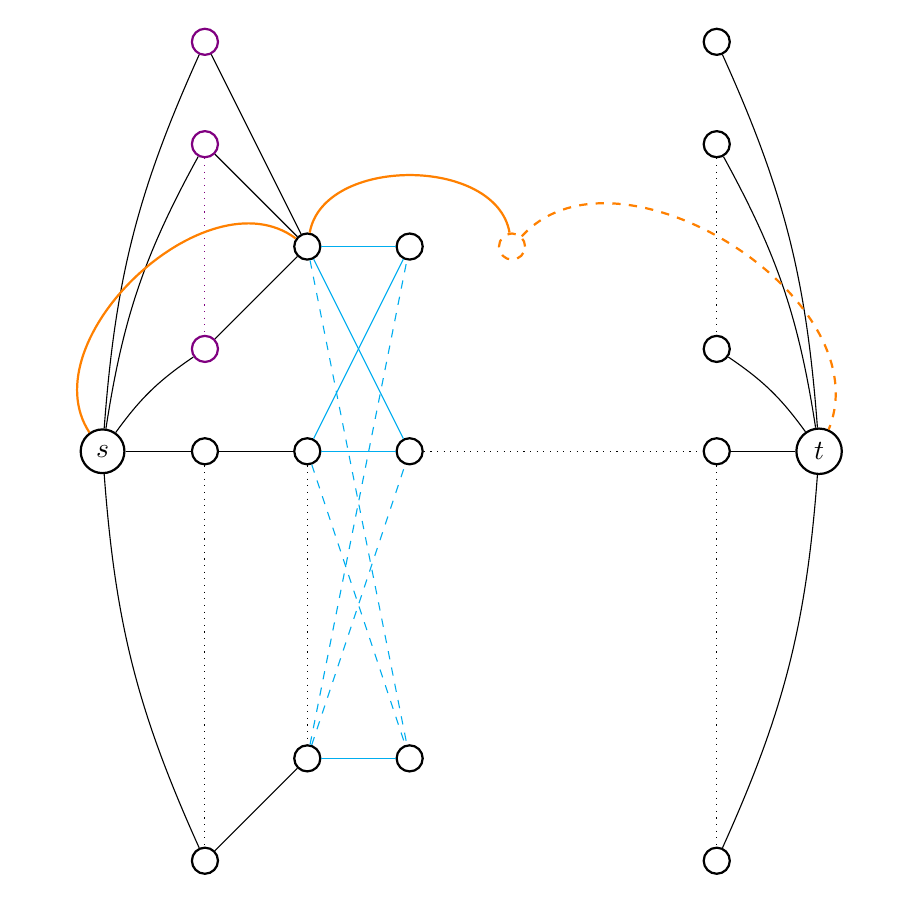
\begin{tikzpicture}[node distance={13mm}, main/.style = {draw, thick, circle}]
		%% Nodes
		\node[main] (s) {$s$};
		% First layer.
		\node[main, right of = s] (2) {};
		\node[main, above of = 2, color = violet] (1l) {};
		\node[above of = 1l] (1phantom) {};
		\node[main, above of = 1phantom, color = violet] (12) {};
		\node[main, above of = 12, color = violet] (11) {};
		\node[below of = 2] (ph1) {};
		\node[below of = ph1] (ph2) {};
		\node[below of = ph2] (ph3) {};
		\node[main, below of = ph3] (last) {};
		% Second layer.
		\node[main, right of = 2] (3) {};
		\node[above of = 3] (ph-layer2-3) {};
		\node[main, above of = ph-layer2-3] (layer21) {};
		\node[below of = 3] (ph-layer2-4) {};
		\node[below of = ph-layer2-4] (ph-layer2-5) {};
		\node[main, below of = ph-layer2-5] (layer2last) {};
		% Third layer.
		\node[main, right of = 3] (4) {};
		\node[main, right of = layer21] (layer31) {};
		\node[main, right of = layer2last] (layer3last) {};
		% Shortcut 4 layer.
		\node[main, dashed, color = orange, right of = layer31] (shortcut) {};
		% Mid layers.
		\node[right of = 4] (5) {};
		\node[right of = 5] (6) {};
		% Last layer.
		\node[main, right of = 6] (7) {};
		\node[main, above of = 7] (7l) {};
		\node[above of = 7l] (7phantom) {};
		\node[main, above of = 7phantom] (72) {};
		\node[main, above of = 72] (71) {};
		\node[below of = 7] (ph7) {};
		\node[below of = ph7] (ph8) {};
		\node[below of = ph8] (ph9) {};
		\node[main, below of = ph9] (last7) {};
		\node[main, right of = 7] (t) {$t$};
		%% Edges.
		\draw (s) edge (2);
		\draw[bend left = 10] (s) edge (11);
		\draw[bend left = 10] (s) edge (12);
		\draw[bend left = 10] (s) edge (1l);
		\draw[bend right = 10] (s) edge (last);
		% Dots.
		\draw[dotted, color = violet] (12) edge (1l);
		\draw[dotted] (2) edge (last);
		% Second layer.
		\draw (2) edge (3);
		\draw (11) edge (layer21);
		\draw (12) edge (layer21);
		\draw (1l) edge (layer21);
		\draw (last) edge (layer2last);
		% Dots.
		\draw[dotted] (3) edge (layer2last);
		% Third layer.
		\draw[color = cyan] (layer21) edge (layer31);
		\draw[color = cyan] (3) edge (layer31);
		\draw[dashed, color = cyan] (layer2last) edge (layer31);
		\draw[dashed, color = cyan] (layer21) edge (layer3last);
		\draw[dashed, color = cyan] (3) edge (layer3last);
		\draw[color = cyan] (layer2last) edge (layer3last);
		\draw[color = cyan] (layer21) edge (4);
		\draw[color = cyan] (3) edge (4);
		\draw[dashed, color = cyan] (layer2last) edge (4);
		% Dots.
		\draw[dotted] (4) edge (7);
		% Last layer.
		\draw (t) edge (7);
		\draw[bend left = 10] (71) edge (t);
		\draw[bend left = 10] (72) edge (t);
		\draw[bend left = 10] (7l) edge (t);
		\draw[bend right = 10] (last7) edge (t);
		% Dots.
		\draw[dotted] (72) edge (7l);
		\draw[dotted] (7) edge (last7);
		% Shortcut.
		\draw[color = orange, bend left = 80, thick] (s) edge (layer21);
		\draw[color = orange, bend left = 80, thick] (layer21) edge (shortcut);
		\draw[color = orange, bend left = 80, thick, dashed] (shortcut) edge (t);
	\end{tikzpicture}
	\caption{Instance of an $L$-cut with integrality gap $n^{2/3}$.}
	\label{huge integrality gap}
\end{figure}

Let $L = 3k$. As in the previous instance at least half of (that is $k$) the shortcut must be used for $L$-flow. Hence the max $L$-flow is at most 2. But one can prove that the following holds. Min $L$-cut is at least $n^{2/3}$. That is we can remove edges between two parts that form complete bipartite graph. This is only a sketch and it does not get into a details.

All in all this particular instance has integrality gap $O(n^{2/3})$.

\section{$L$-flow}

In this section we will take a look at an algorithm for $L$-flow that would be fast and won't used \textbf{LP}. As it turns out there is as of now only an approximation scheme, which is fully polynomial time approximation scheme (FPTAS for short). Now $y(e)$ is the value for min cut in (\textbf{D}) and $c(e)$ the capacity for edge $e$. Then $x(p)$ is the same as $f_p$ in (\textbf{P}).

\begin{algorithm}
	\caption{FPTAS for $\max L$-flow}
	\begin{algorithmic}[1]
		\Require $G = (V,E)$
		\Ensure $\max L$-bounded flow.
		\State $\epsilon > 0$ $\forall e \in E$, $\delta = \delta(\epsilon)$ $\forall p \in \mathcal{P}_L$
		\While{the $y$-shortest path $p \in \mathcal{P}_L$ has length $< 1$}
			\State $c = \min_{e \in p} c(e)$
			\State $x(p) = x(p) + \epsilon$
			\State $y(e) = y(e) \left( 1 + \frac{\epsilon c}{c(e)} \right)$ $\forall e \in p$
		\EndWhile
		\State \Return $x$
	\end{algorithmic}
\end{algorithm}

\begin{lemma}
	$x$ scaled down by $\log_{1 + \epsilon} \frac{1+\epsilon}{\delta}$ is a feasible solution.
\end{lemma}

\begin{thm}
	The scaled flow is $(1 + \epsilon)$-approximation.
\end{thm}

Few remarks. Firstly this algorithm can be done by using Dijkstra's algorithm on the layered graph, which is similiar to the one already mentioned. That is $L$ layers and finding shortest path from $(s,0)$ to $(t, L)$. Other remark is that indeed this does not use LP.

Sometimes this type of algorithm is called \textit{Multiplicative weight update algorithm}. Which can also be applied for the multi-commodity flow. Intuitively the algorithm avoids heavily used edges and prefer spreading the flows.
\end{document}

